% !TeX encoding = UTF-8
% !TeX root = V34_TEM.tex
% !TeX spellcheck = de_DE_frami

\section{Durchführung}

\subsection{Vorversuch optische Abbildungen}
Die Funktionsweise und Messmodi eines Elektronenmikroskops lassen sich anschaulich am Modell des Lichtmikroskops zeigen. Als Lichtquelle dient uns ein Laser, dessen Strahl durch eine Aufweitungsoptik aus zwei Linsen $L_1, L_2$ mit Brennweiten $f_1, f_2$ und Abstand $f_1 + f_2$ verbreitert wird. Dabei bündelt $L_1$ den Laserstrahl im Brennpunkt zwischen den Linsen, der als Punktquelle für $L_2$ dient und erneut parallelisiert wird. Gemäß dem Strahlensatz wird der Strahl dabei um den Faktor $\frac{f_2}{f_1}$ aufgeweitet, wodurch ein großer Bereich gleichmäßig ausgeleuchtet werden kann.

Nun werden verschiedene Objekte O durch zwei Linsen (Objektiv $L_3$, Okular $L_4$) auf die Wand $B$ abgebildet. Das Objektiv wird anschließend so verschoben, dass das Beugungsbild von O mit $g = \infty$ abgebildet wird.

\begin{figure}[h]
	\centering
	\def\svgwidth{0.75\textwidth}
	\input{graphics/light.pdf_tex}
	\caption{Zeichnung Lichtmikroskop, Abbildung des Objektes}
	\label{fig:light}
\end{figure}


\subsubsection{Spalte und Gitter}
\enlargethispage{2\baselineskip}

\begin{figure}[p]
	\centering
	\begin{subfigure}[b]{0.49\textwidth}
		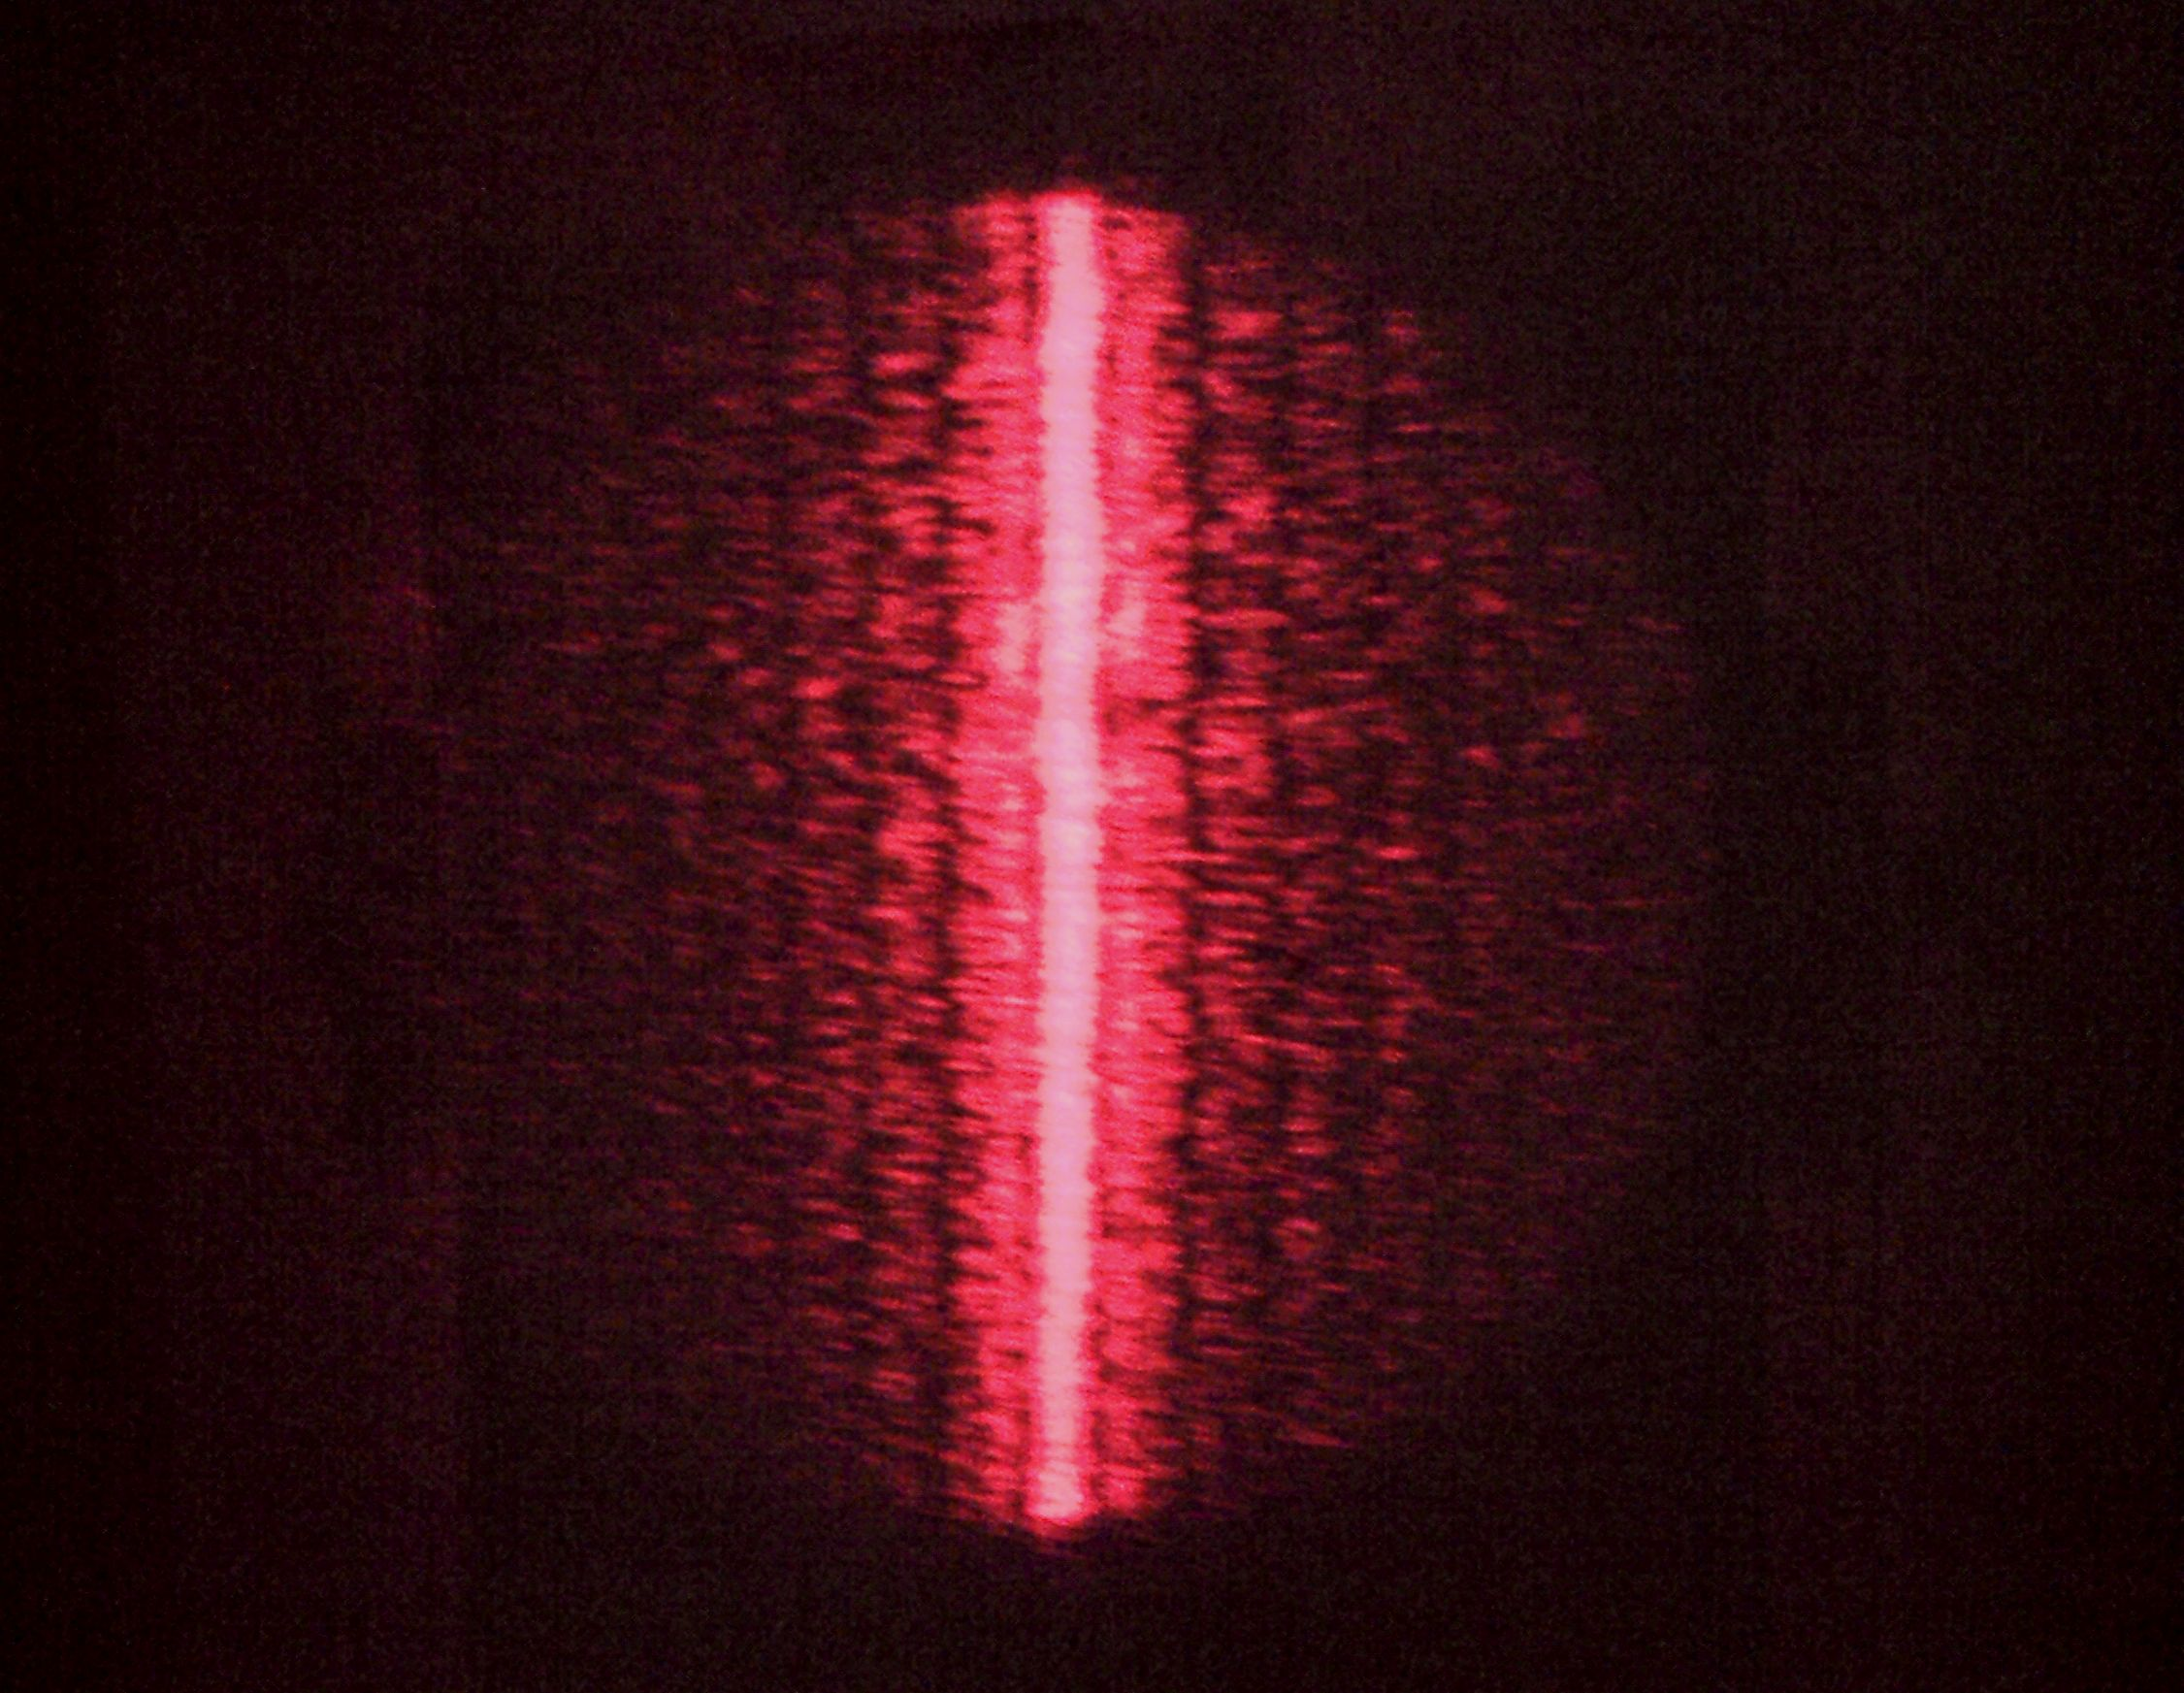
\includegraphics[width=\textwidth]{data/optics/02_Einzelspalt_Bild}
		\caption{Bild}
	\end{subfigure}
	\begin{subfigure}[b]{0.49\textwidth}
		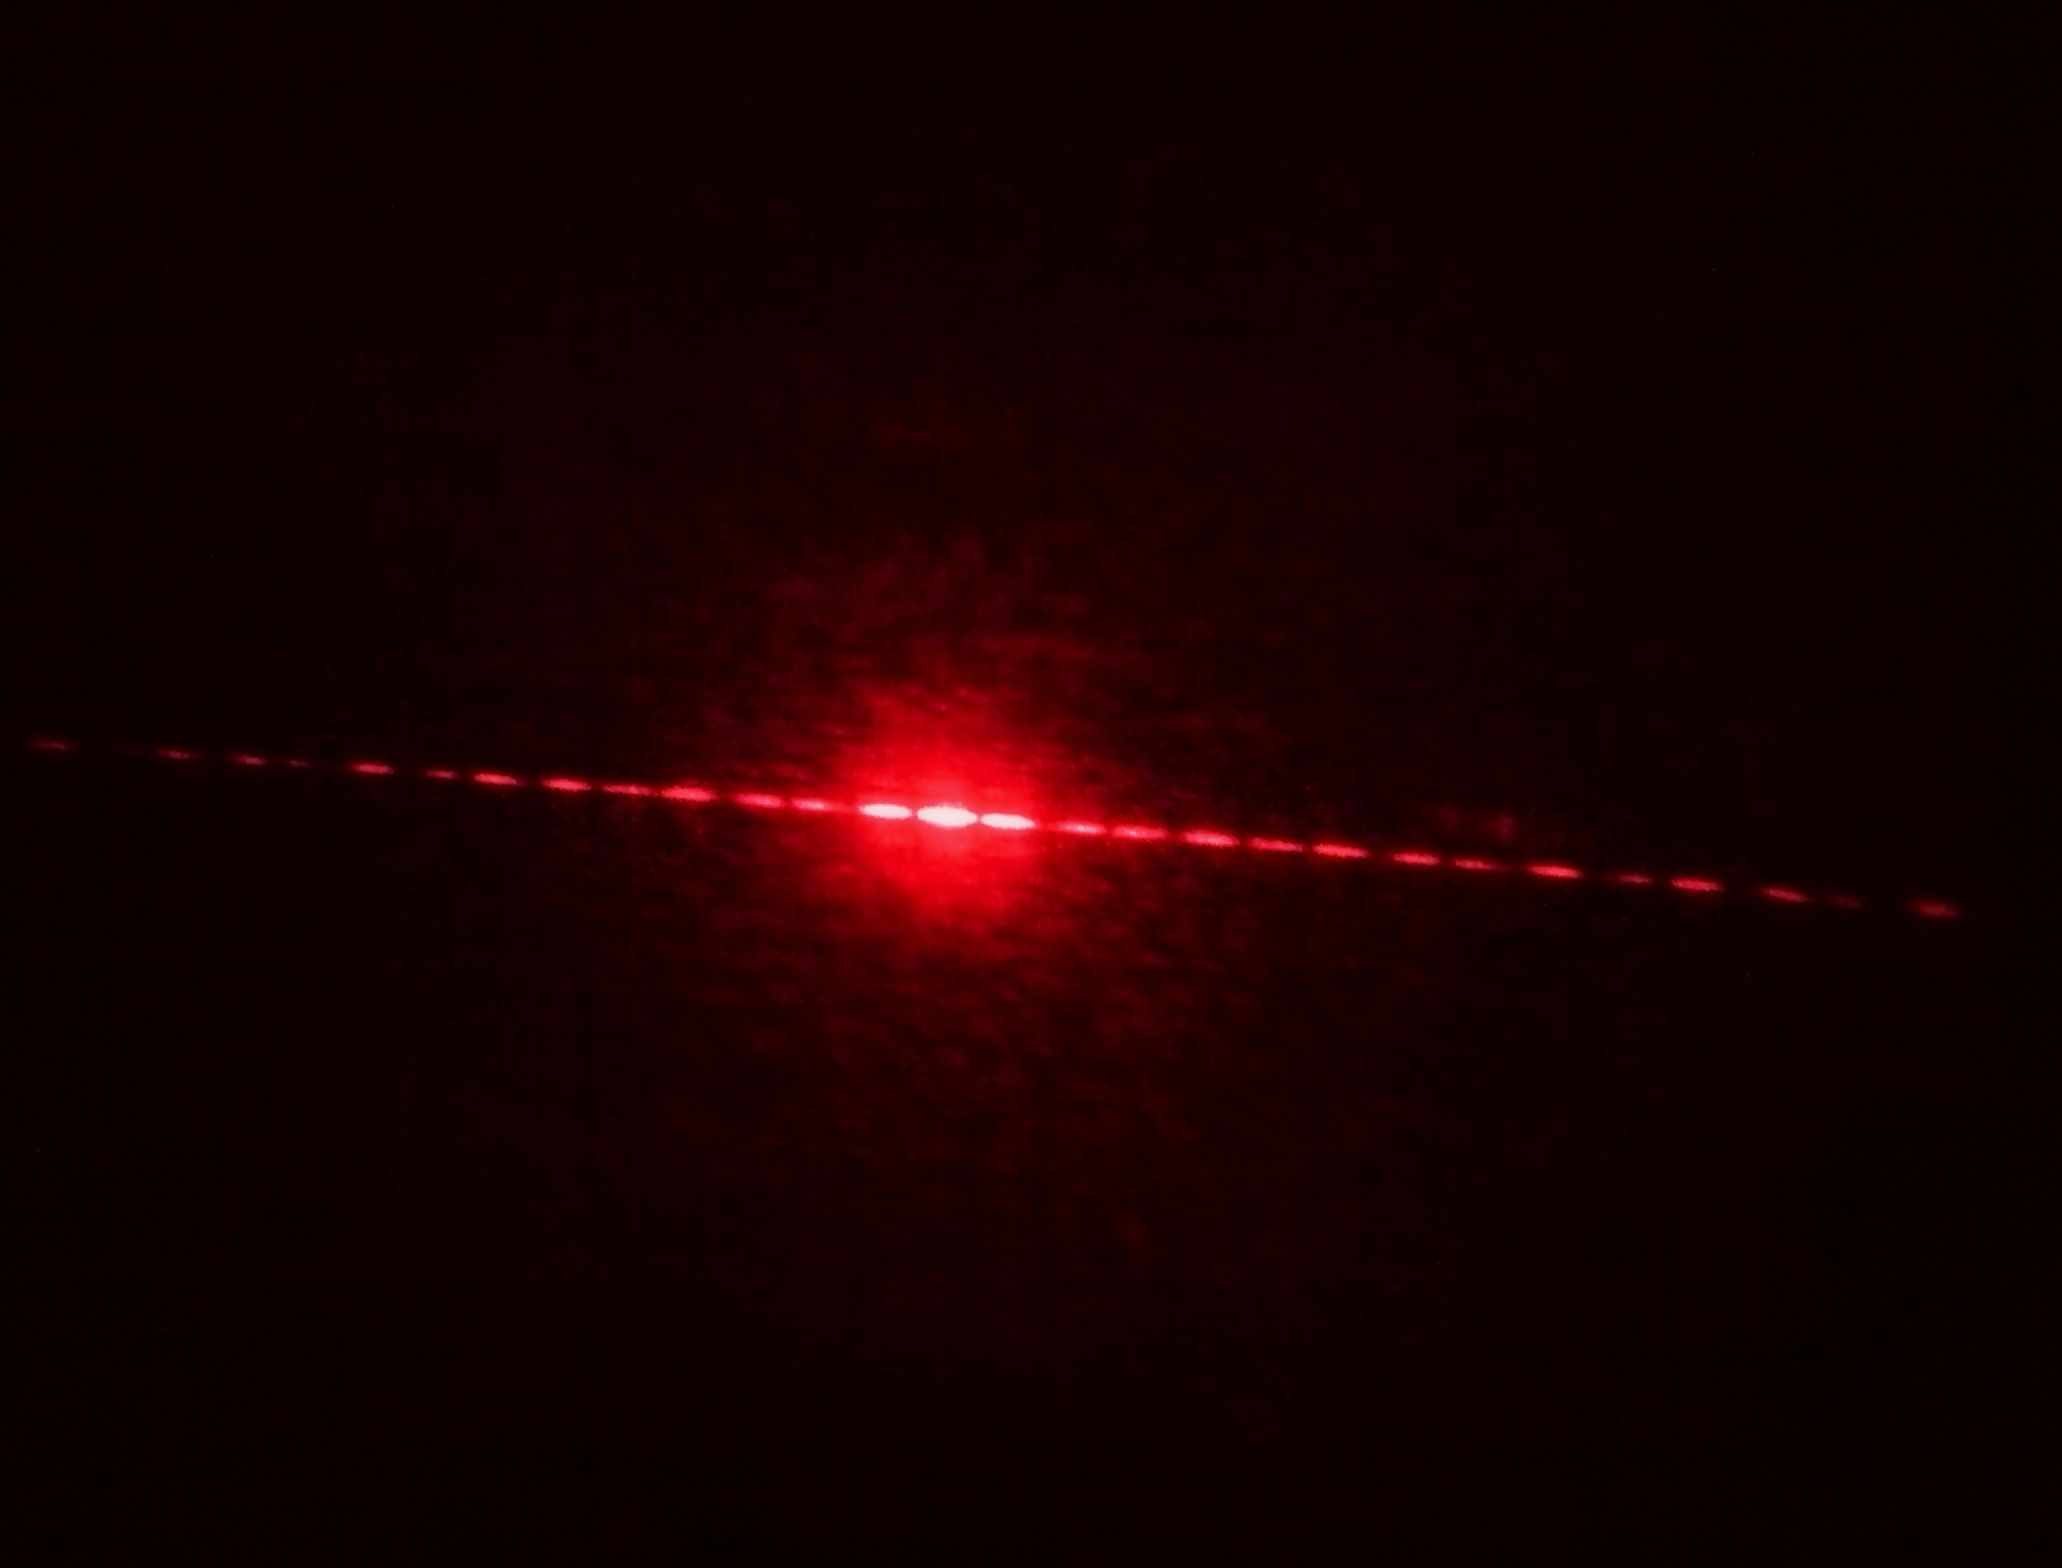
\includegraphics[width=\textwidth]{data/optics/02_Einzelspalt_Beugung}
		\caption{Beugungsbild} 		\label{fig:Einzel_BG}
	\end{subfigure}
	\caption{Einzelspalt}				\label{fig:Einzel}
	\vspace{-1em}
\end{figure}

\begin{figure}[p]
	\centering
	\begin{subfigure}{0.49\textwidth}
		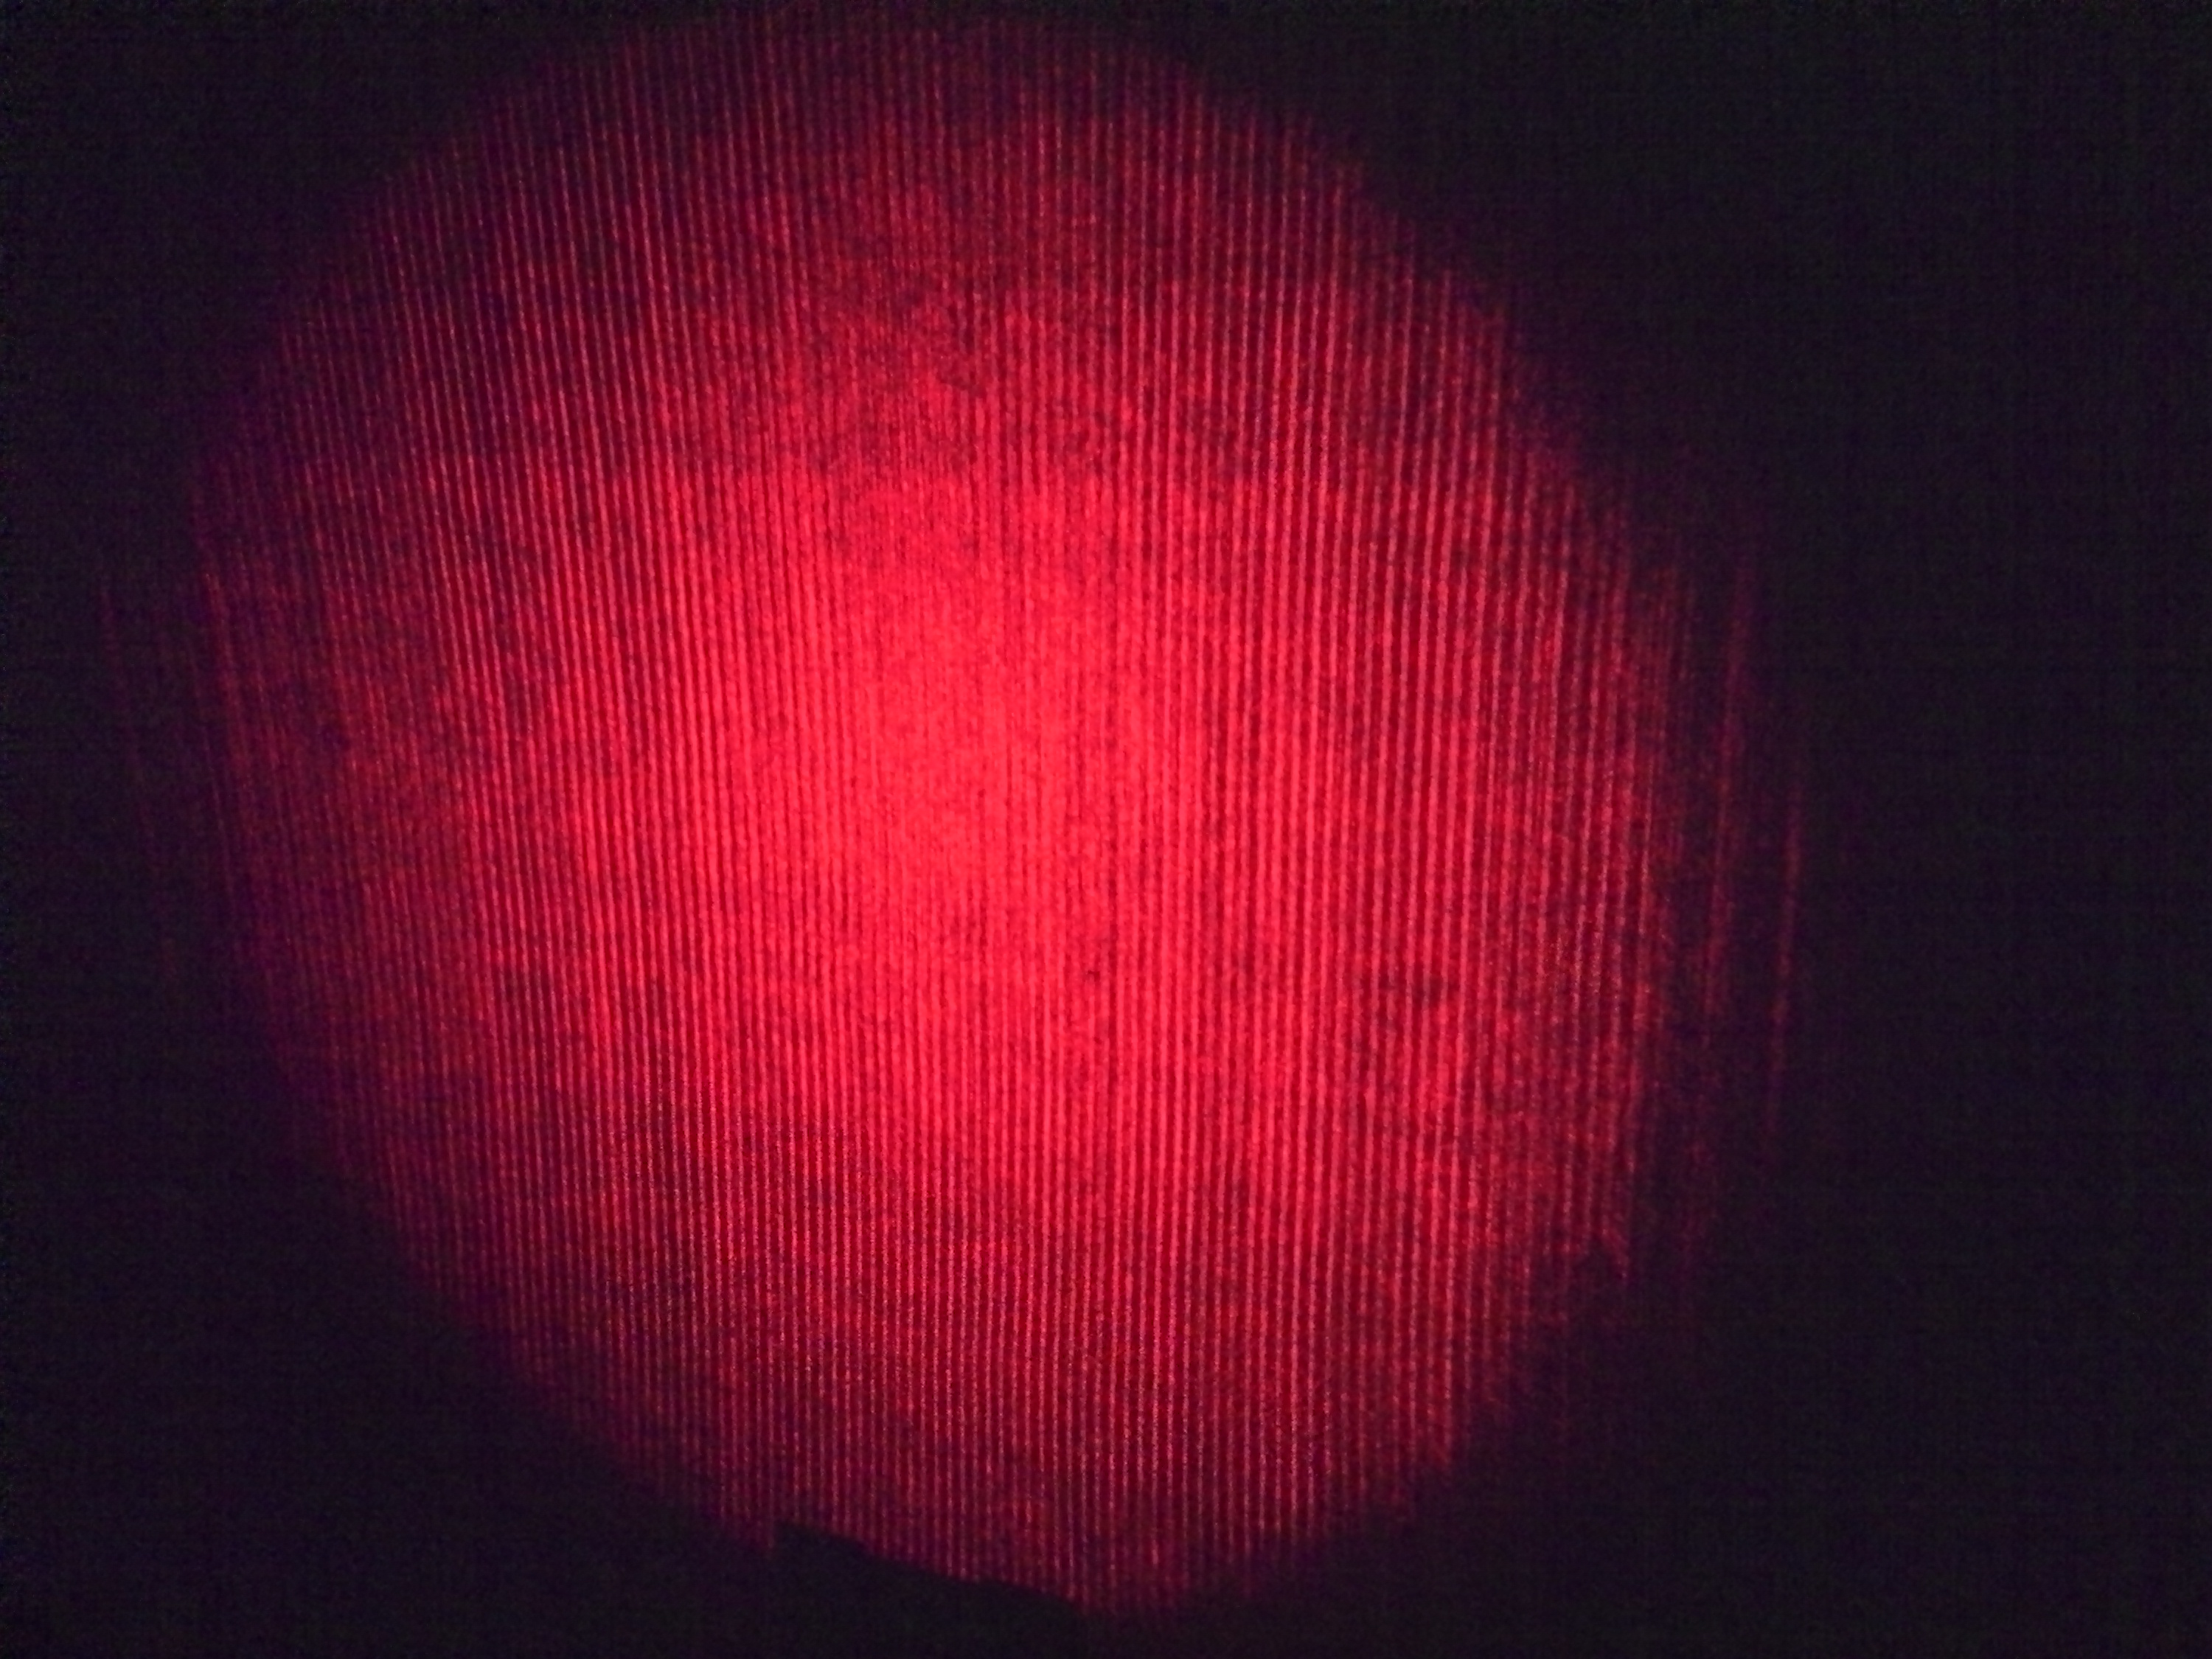
\includegraphics[width=\textwidth]{data/optics/04_Gitter_1D}
		\caption{Bild}
	\end{subfigure}
	\begin{subfigure}{0.49\textwidth}
		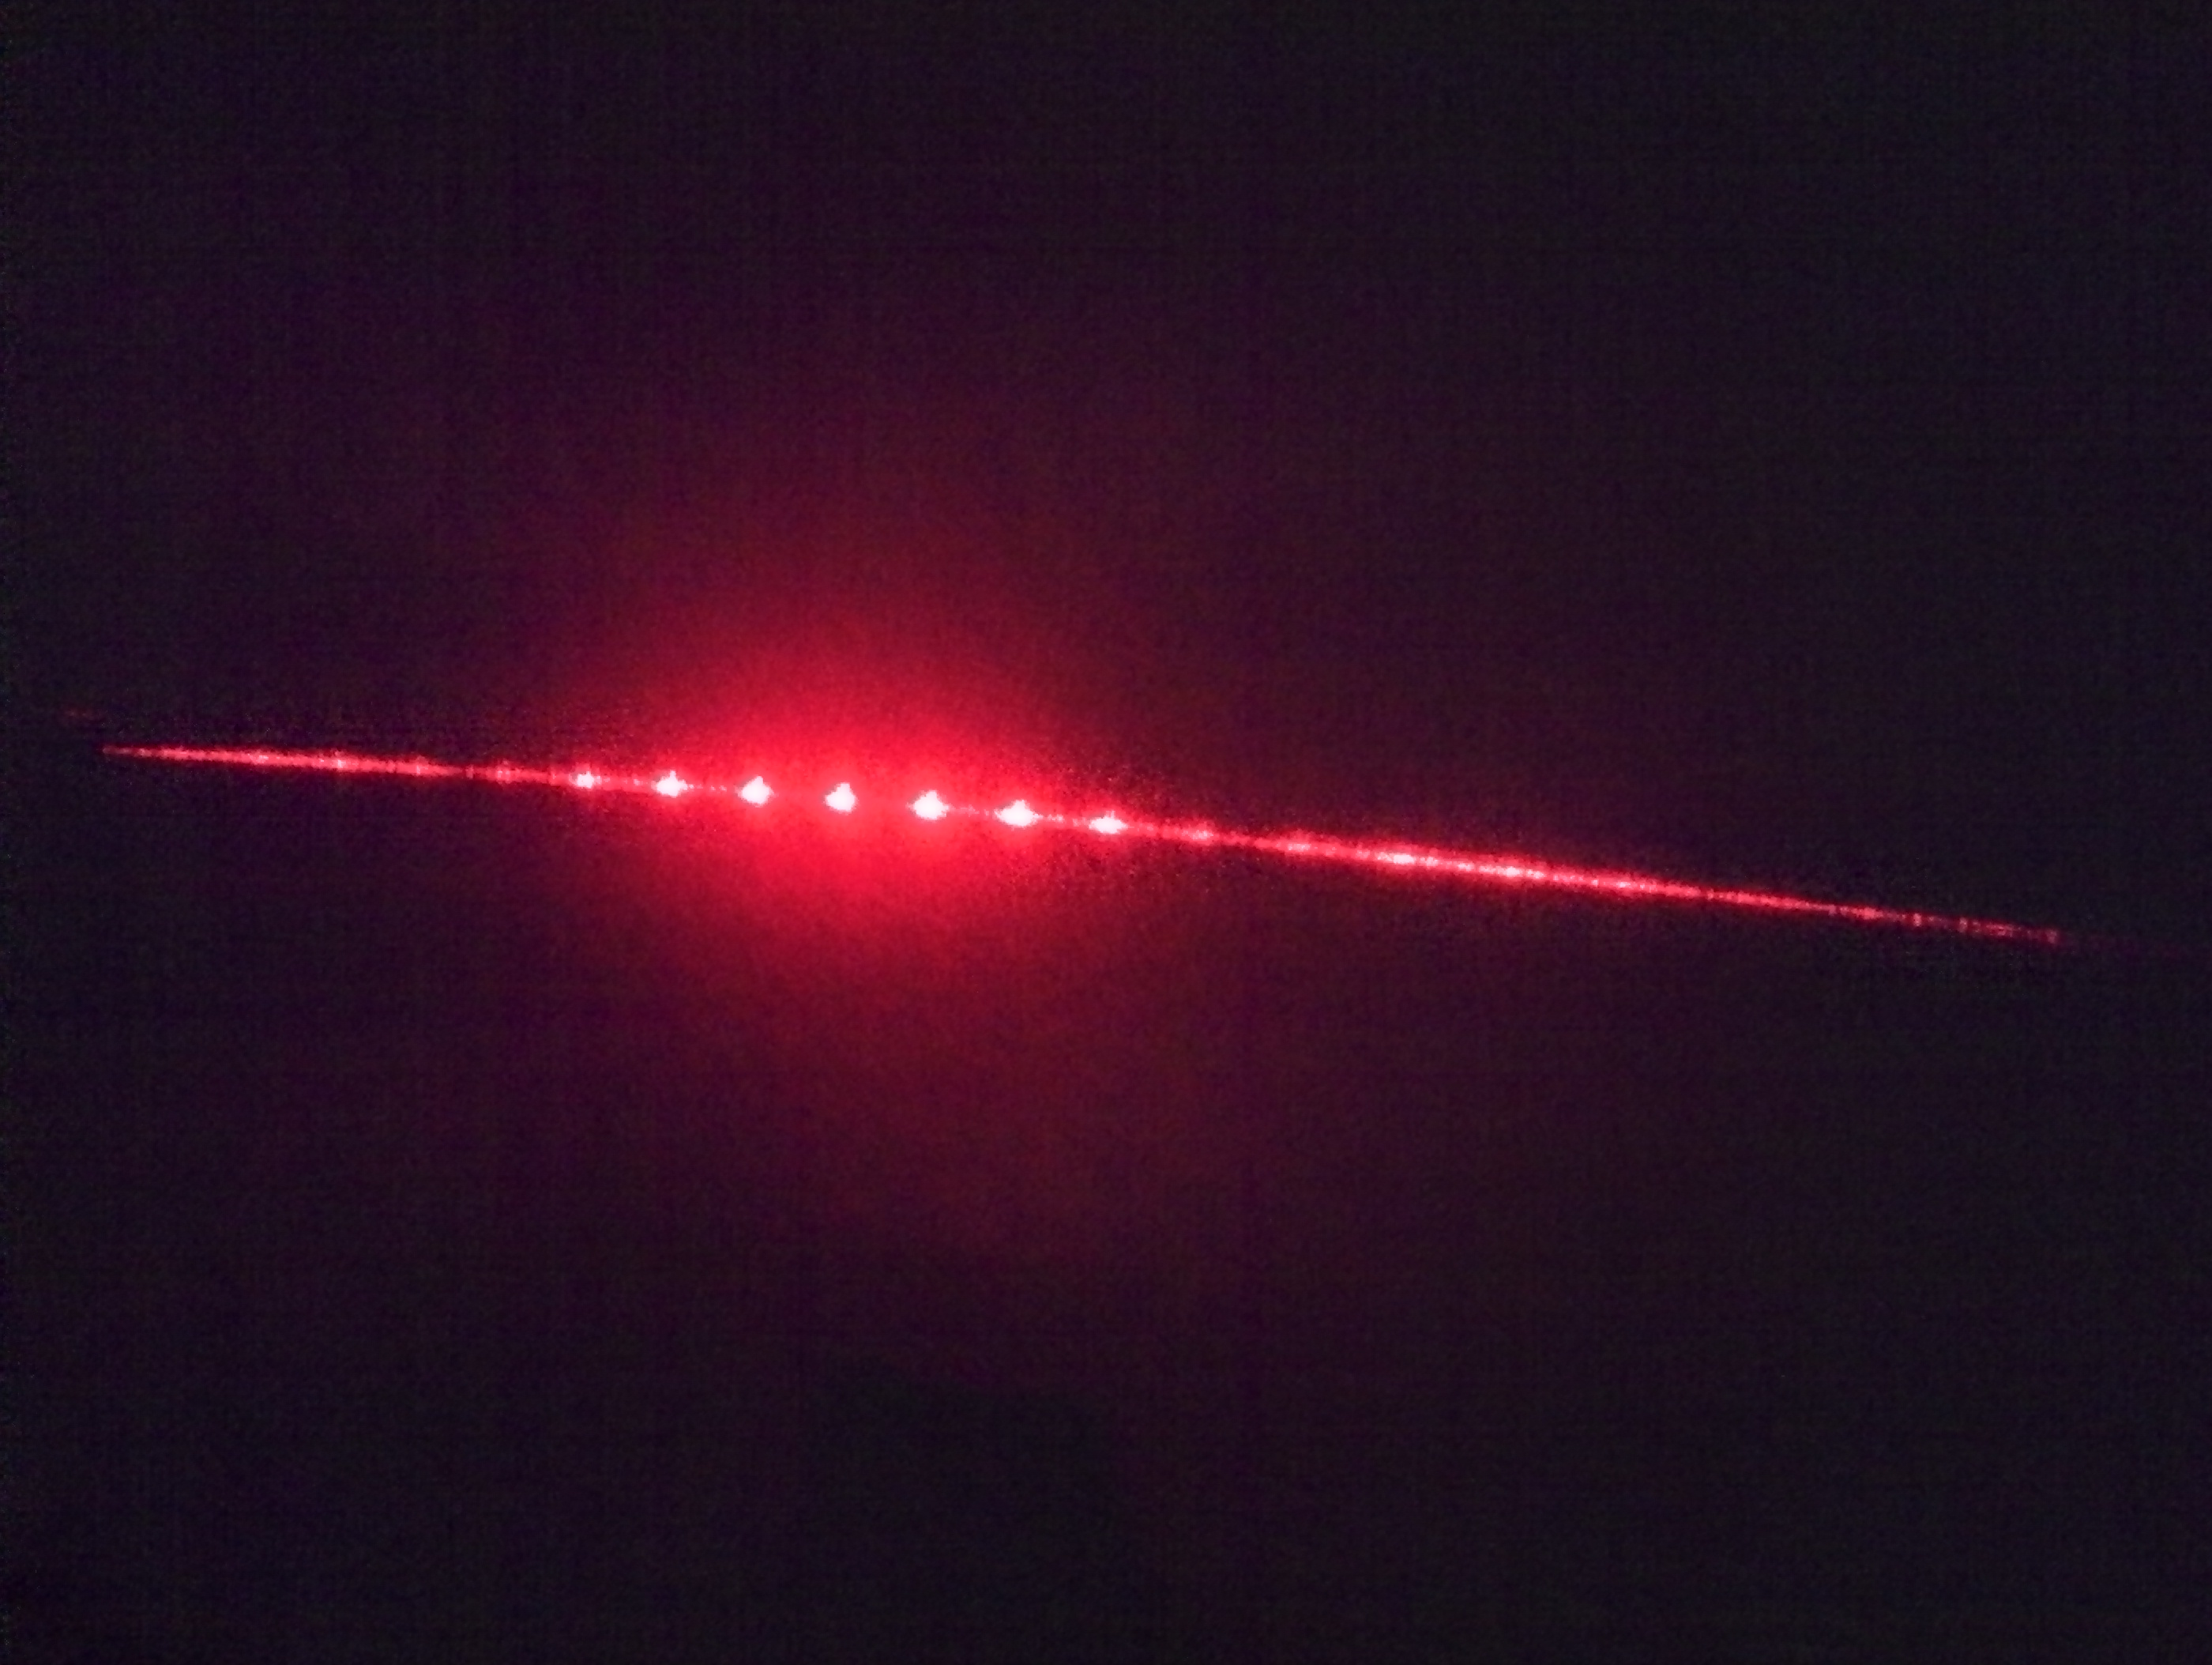
\includegraphics[width=\textwidth]{data/optics/04_Gitter_1D_Beugung}
		\caption{Beugungsbild} 		\label{fig:Gitter_BG}
	\end{subfigure}
	\caption{eindimensionales Gitter}		\label{fig:Gitter}
	\vspace{-1em}
\end{figure}

\begin{figure}[p]
	\centering
	\begin{subfigure}{0.49\textwidth}
		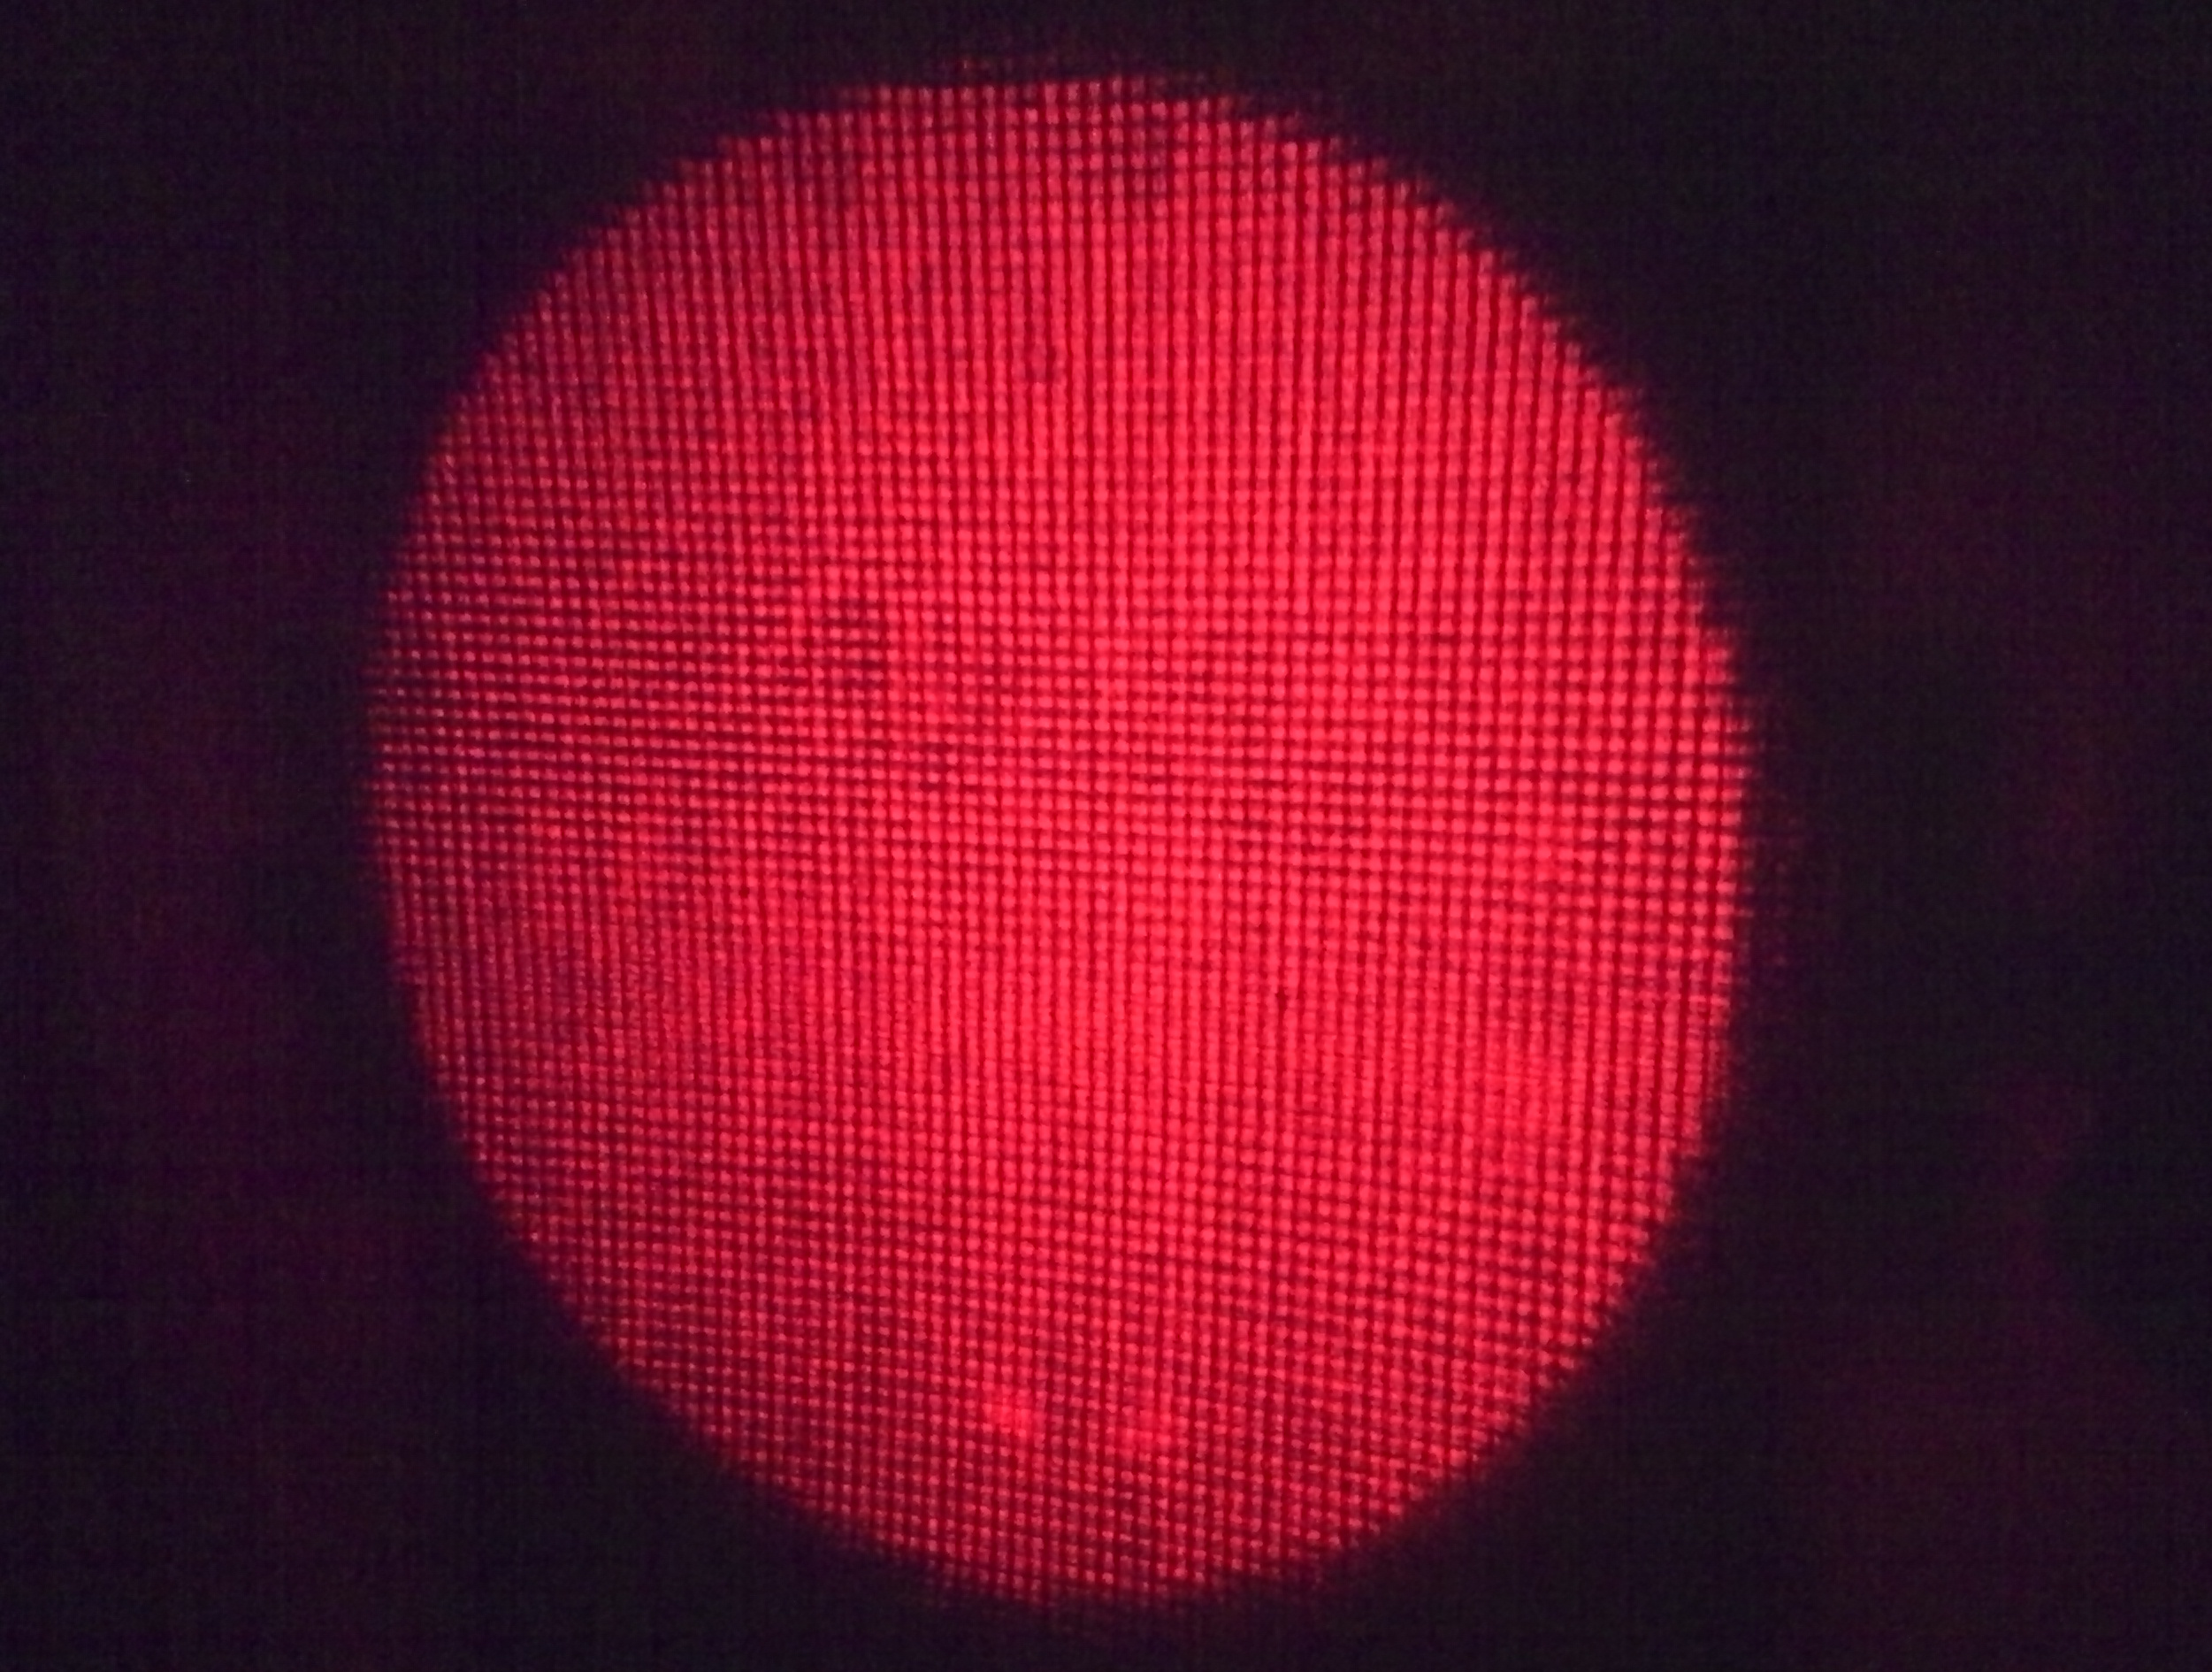
\includegraphics[width=\textwidth]{data/optics/05_Gitter_2D}
		\caption{Bild}
	\end{subfigure}
	\begin{subfigure}{0.49\textwidth}
		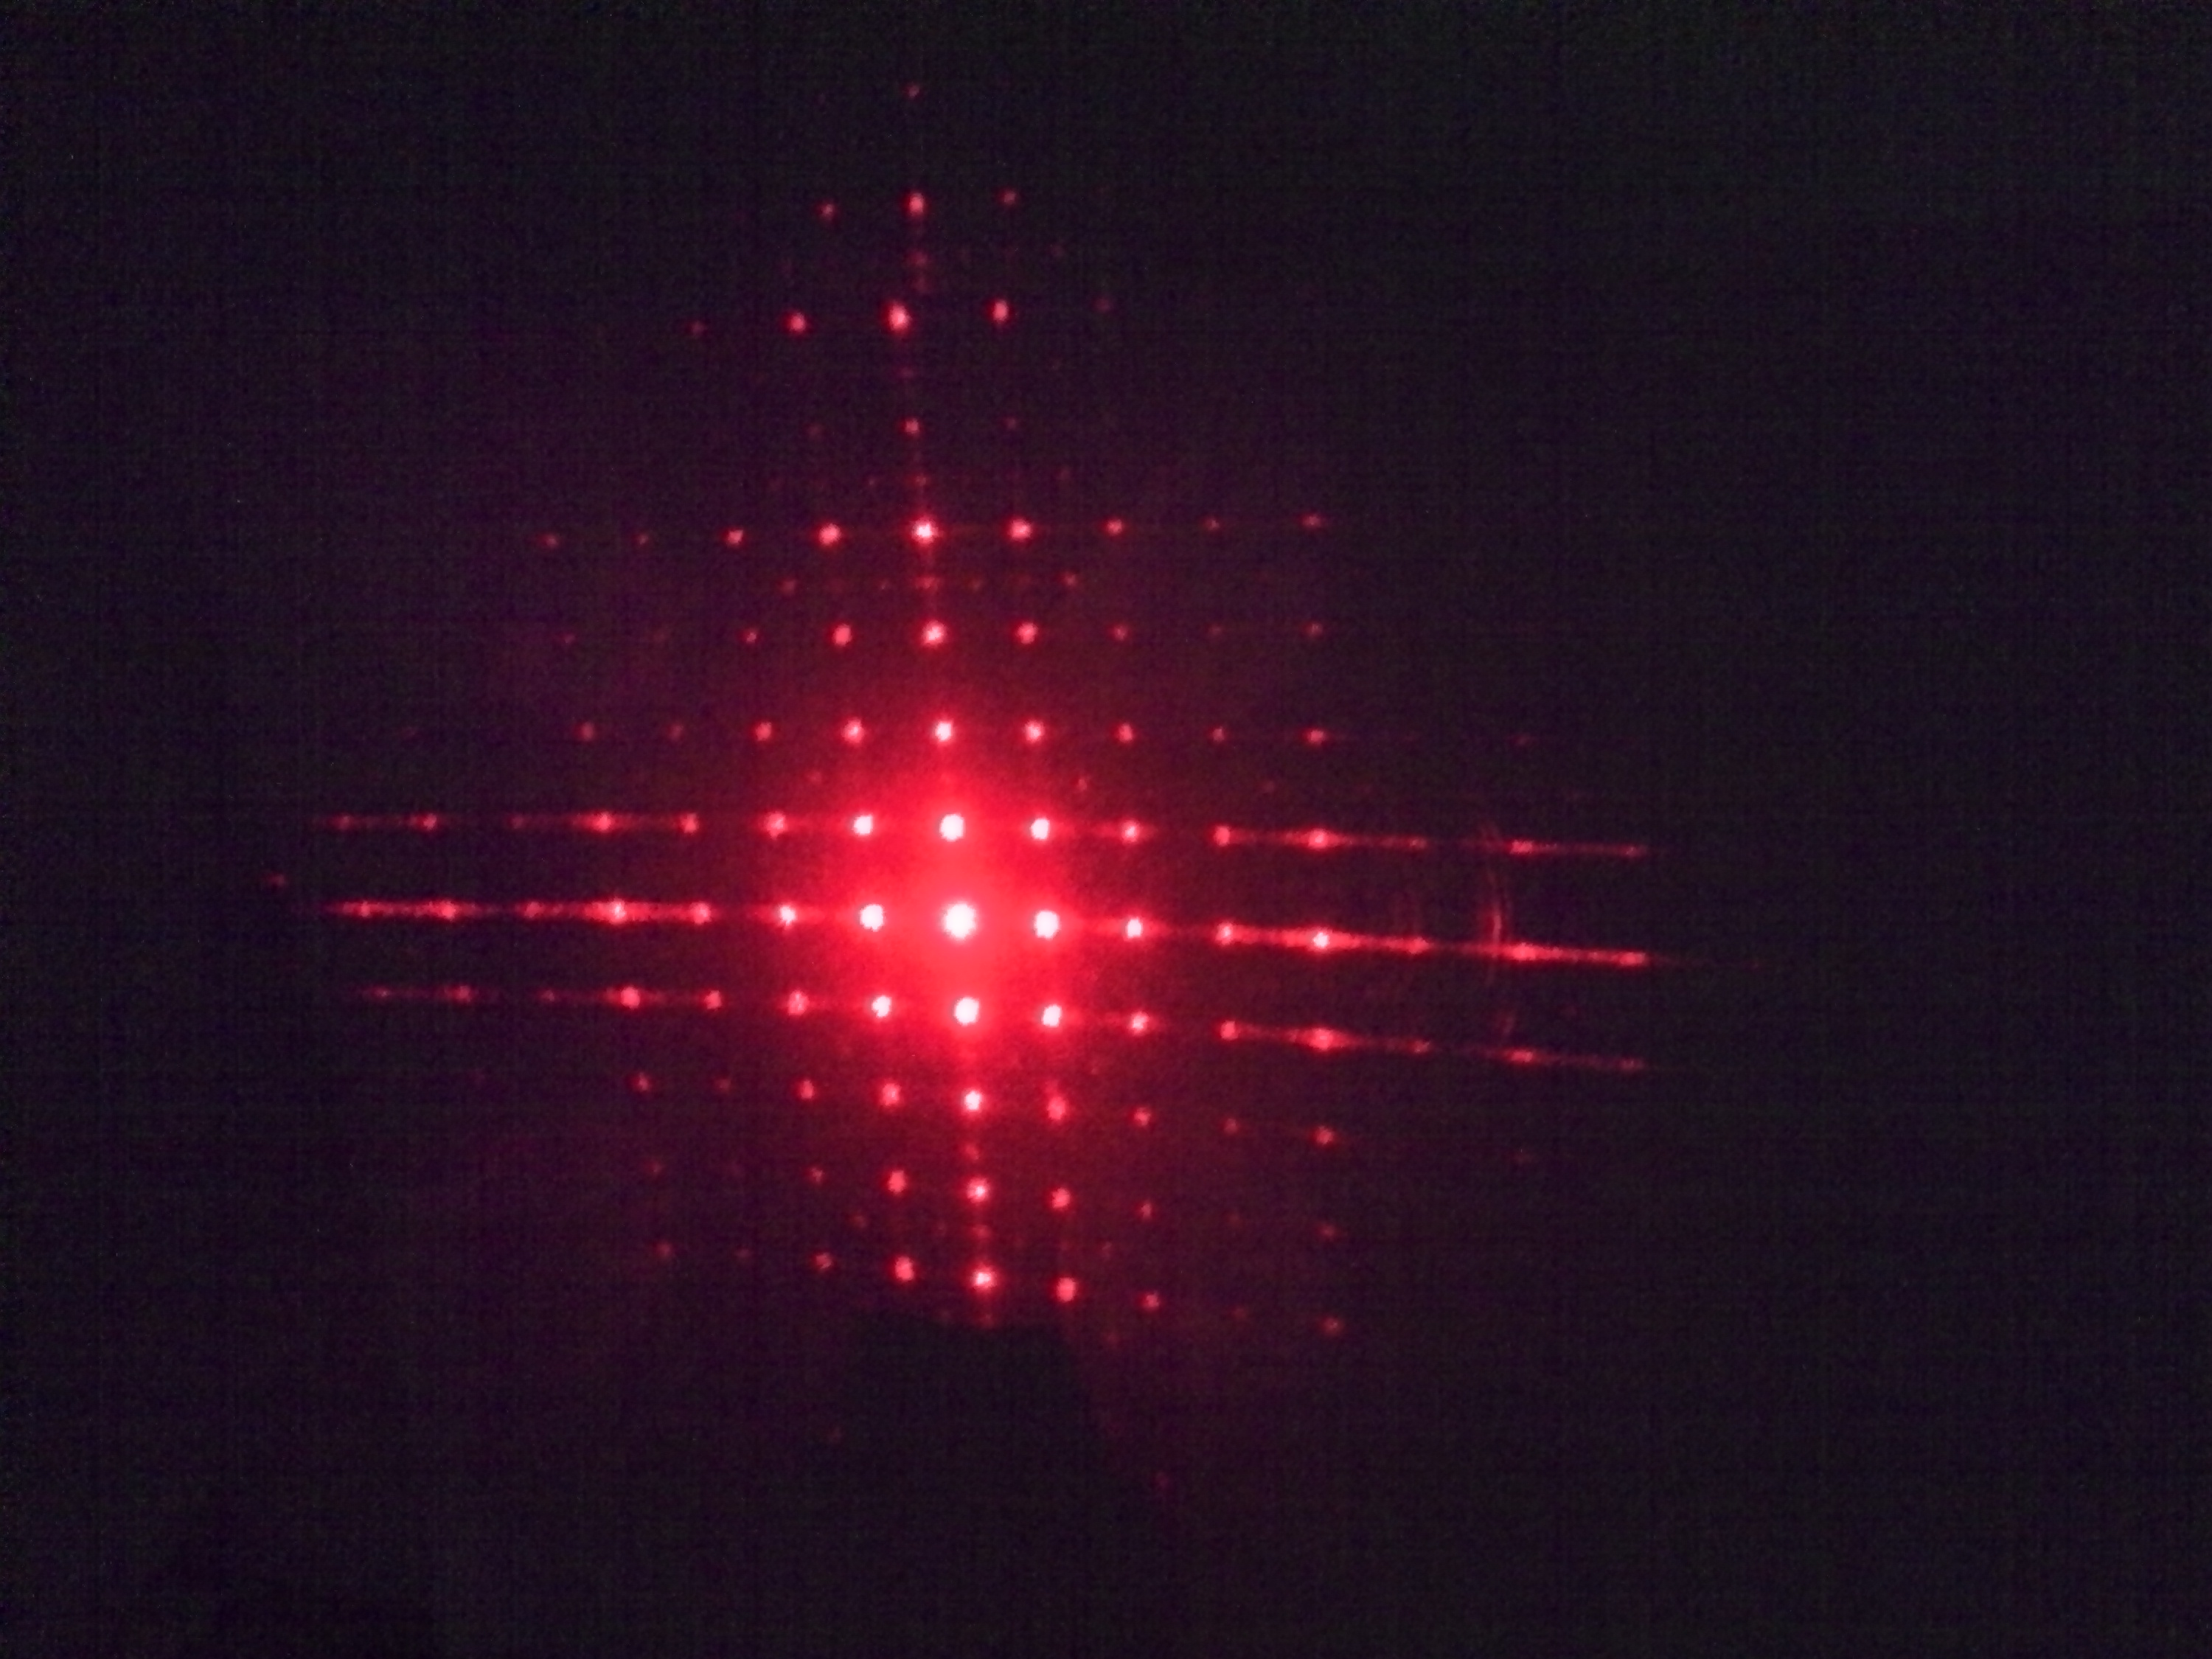
\includegraphics[width=\textwidth]{data/optics/05_Gitter_2D_Beugung}
		\caption{Beugungsbild}		 \label{fig:Gitter_2D_BG}
	\end{subfigure}
	\caption{zweidimensionales Gitter}	\label{fig:Gitter_2D}
	\vspace{-5em}
\end{figure}

Für den Einzelspalt erwarten wir als Intensitätsverlauf im Beugungsbild gemäß Gleichung \eqref{eq:sinc} den Sinus Cardinalis. Das charakteristische Merkmal, das breite Hauptmaximum, ist in unserem Photo jedoch nicht richtig erkennbar (siehe Abb. \ref{fig:Einzel_BG}). Wir vermuten, dass dies am Spalt selbst liegt -- als wir diesen gegen das Licht hielten, war eine schwache zweite Linie erkennbar. Bei einem Doppelspalt wäre das Hauptmaximum gleich breit wie die Nebenmaxima, was das beobachtete Muster erklären würde.

Das Beugungsbild eines perfekten Gitters wäre ein Delta-Kamm, durch die endliche Spaltbreite ist diesem eine $\sinc$-Funktion als Hüllkurve überlagert (Abb. \ref{fig:Gitter_BG}). Da wir den reziproken Raum abbilden, sind kleine Strukturen im Beugungsbild groß und umgekehrt -- da die Spaltbreite deutlich kleiner ist als der Spaltabstand, ist die Hüllkurve breit gegenüber dem Abstand der Maxima.

Das 2D-Gitter ist die Überlagerung zweier 1D-Gitter, somit ist das Beugungsbild ein Punktgitter entlang zweier Achsen (Abb. \ref{fig:Gitter_2D_BG}). Aus diesem ist anhand der gleichen Abstände erkennbar, dass die zwei Gitterkonstanten gleich sind (Netz mit quadratischen Maschen).


\newpage
\subsubsection{Einstein-Portrait}
Auf einem Dia ist das Portrait Einsteins abgebildet, allerdings ist dieses durch ein Gitter überlagert, wodurch man nur ein verschwommenes Bild erhält (Abb. \ref{fig:Einstein_B}). Da das Gitter deutlich feiner ist als das Portrait, zeigen sich im Beugungsbild die typischen Punktreflexe eines Gitters (Abb. \ref{fig:Einstein_BG}). Gemäß dem Faltungstheorem enthält jeder dieser Reflexe die Information des Portraits.

Selektieren wir durch eine Rechteckblende im Brennpunkt von $L_3$ ausschließlich das Hauptmaximum (Abb. \ref{fig:Einstein_hell_B}), so entfällt die Information des Gitters und erhalten ein gefiltertes Bild. Diese Methode wird als Hellfeld-Mikroskopie bezeichnet.

Verschieben wir die Rechteckblende so, dass lediglich das Licht eines Nebenmaximums hindurch gelangt (Abb. \ref{fig:Einstein_dunkel_B}), so sehen wir im Bild nur das am Objekt gestreute Licht und sehen folglich das Portrait auf dunklem Hintergrund, daher auch der Name Dunkelfeld-Mikroskopie. Der Kontrast ist typischerweise besser, allerdings ist die Intensität des gestreuten Lichts verständlicherweise deutlich geringer als im Hellfeld.

\begin{figure}[p]
	\centering
	\begin{subfigure}[b]{0.49\textwidth}
		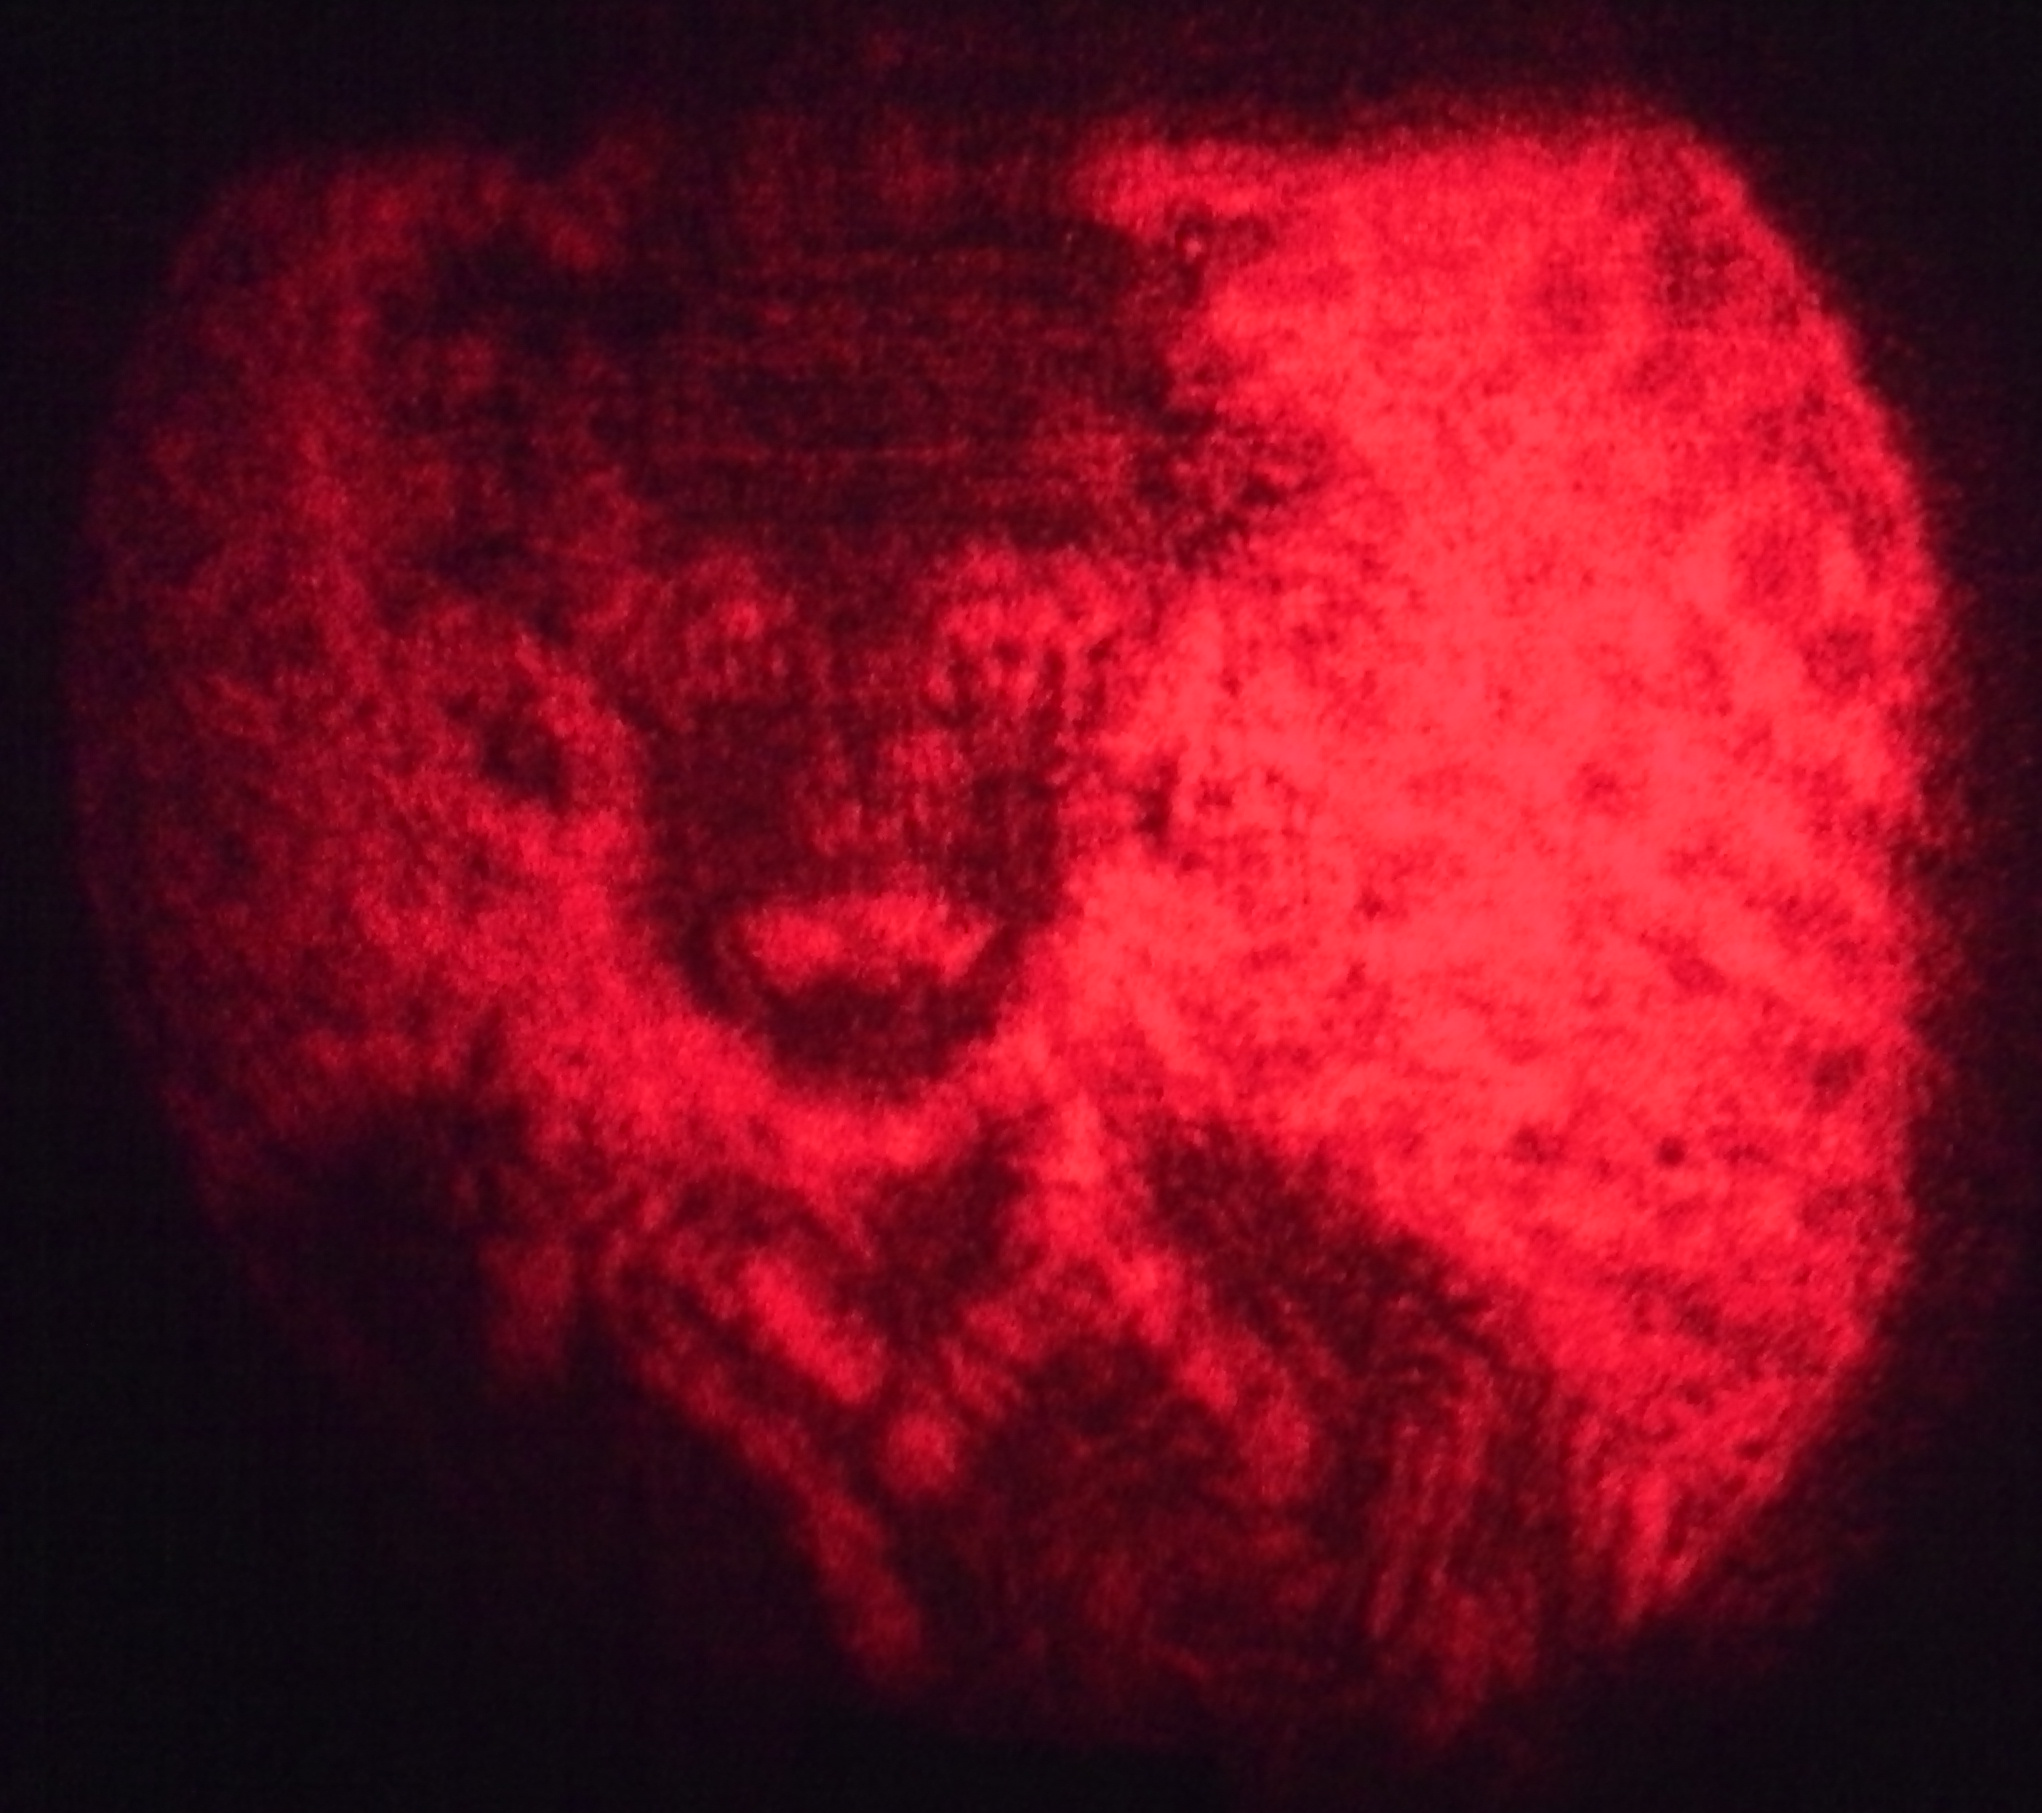
\includegraphics[width=\textwidth]{data/optics/06_Einstein_Bild}
		\caption{Bild}				\label{fig:Einstein_B}
	\end{subfigure}
	\begin{subfigure}[b]{0.49\textwidth}
		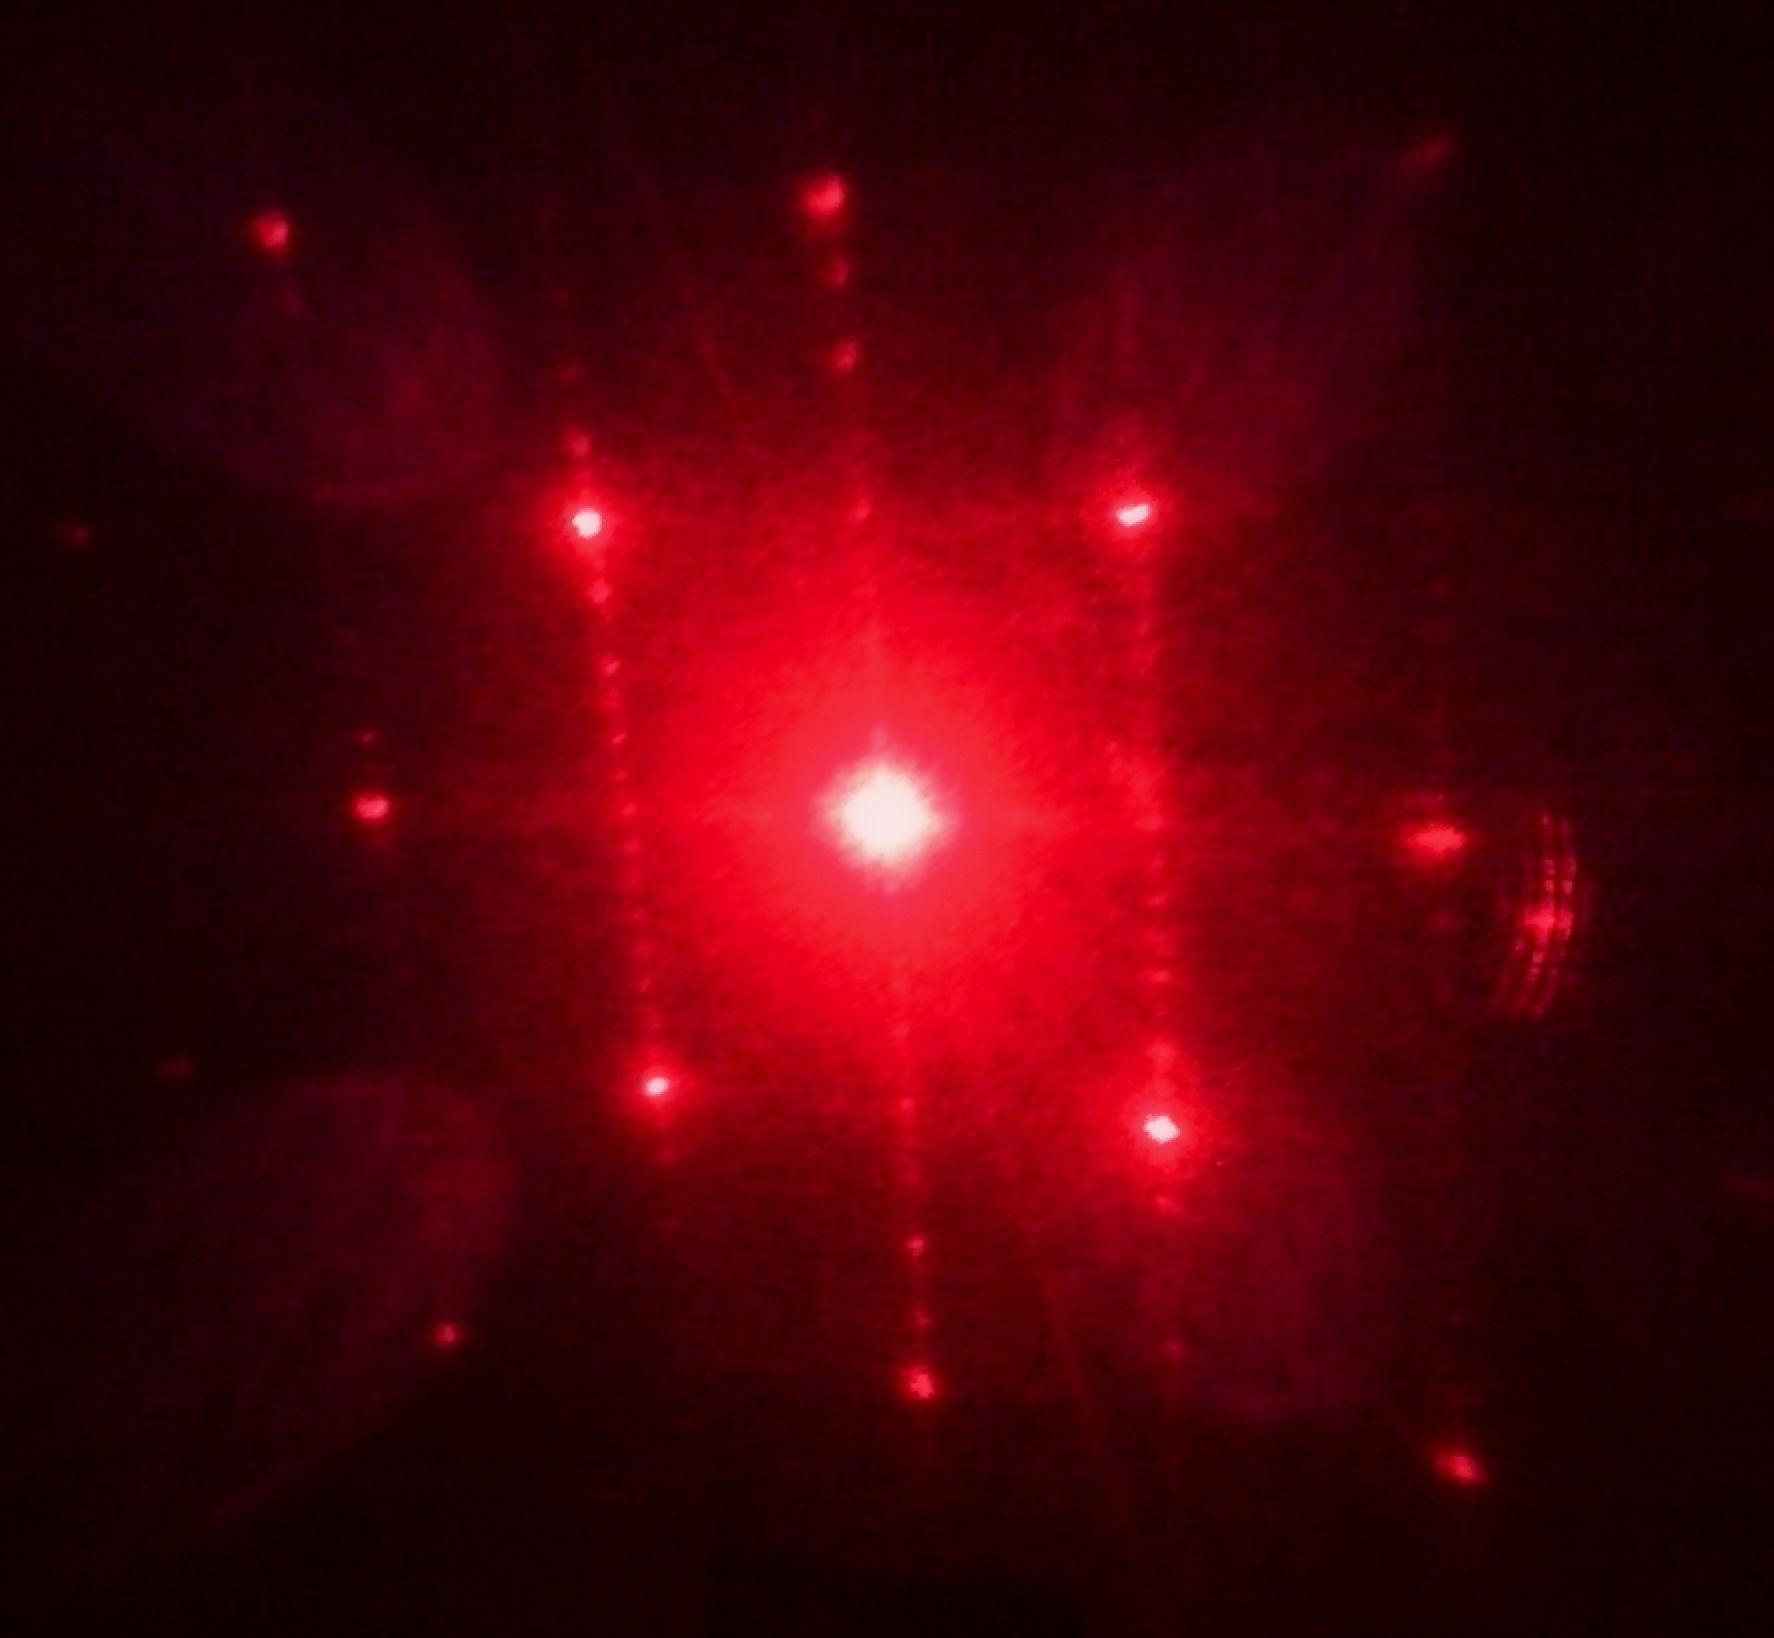
\includegraphics[width=\textwidth]{data/optics/06_Einstein_Beugung}
		\caption{Beugungsbild} 		\label{fig:Einstein_BG}
	\end{subfigure}
	\caption{Einstein-Portrait}			\label{fig:Einstein}
	\vspace{-1em}
\end{figure}

\begin{figure}[p]
	\centering
	\begin{subfigure}{0.49\textwidth}
		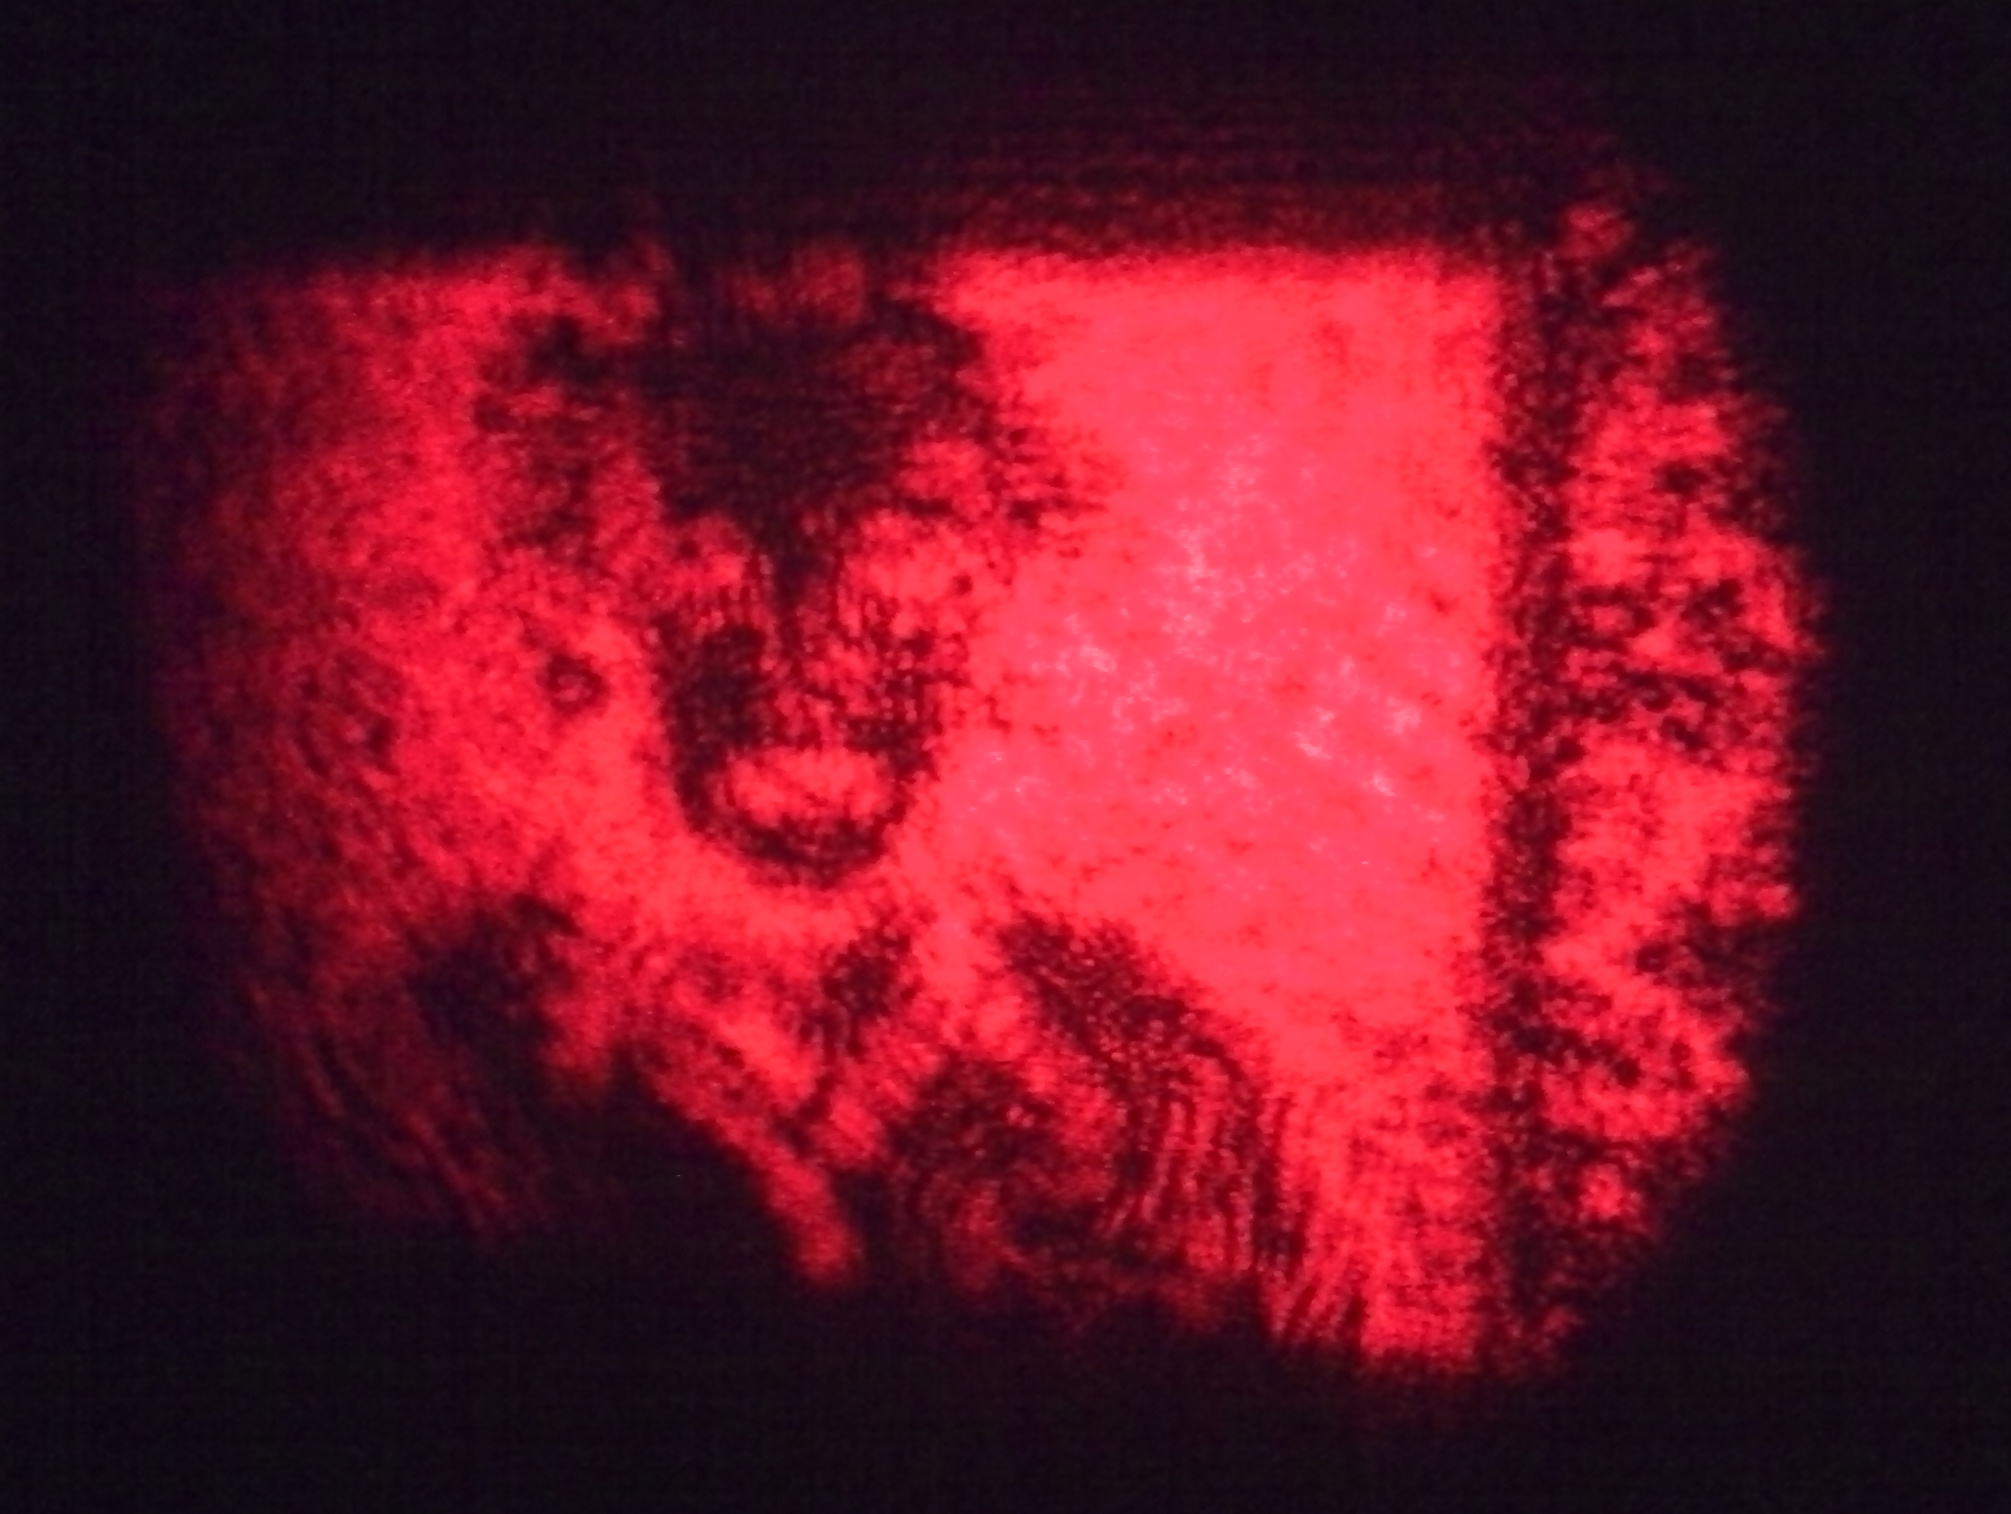
\includegraphics[width=\textwidth]{data/optics/06_Einstein_Hell_Bild}
		\caption{Hellfeld-Bild}				\label{fig:Einstein_hell_B}
	\end{subfigure}
	\begin{subfigure}{0.49\textwidth}
		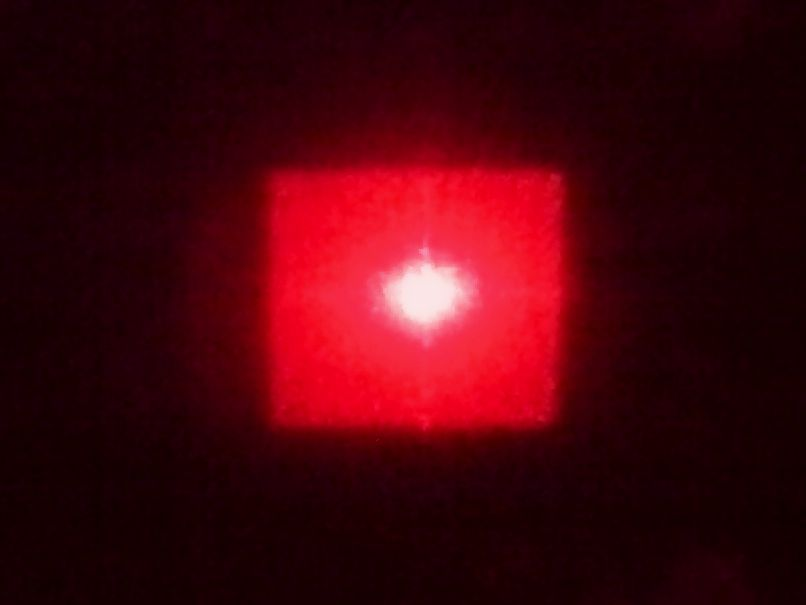
\includegraphics[width=\textwidth]{data/optics/06_Einstein_Hell_Beugung}
		\caption{Beugungsbild: Hauptmaximum}	\label{fig:Einstein_hell_BG}
	\end{subfigure}
	\caption{Einstein-Portrait im Hellfeld}		\label{fig:Einstein_hell}
	\vspace{-1em}
\end{figure}

\begin{figure}[p]
	\centering
	\begin{subfigure}{0.49\textwidth}
		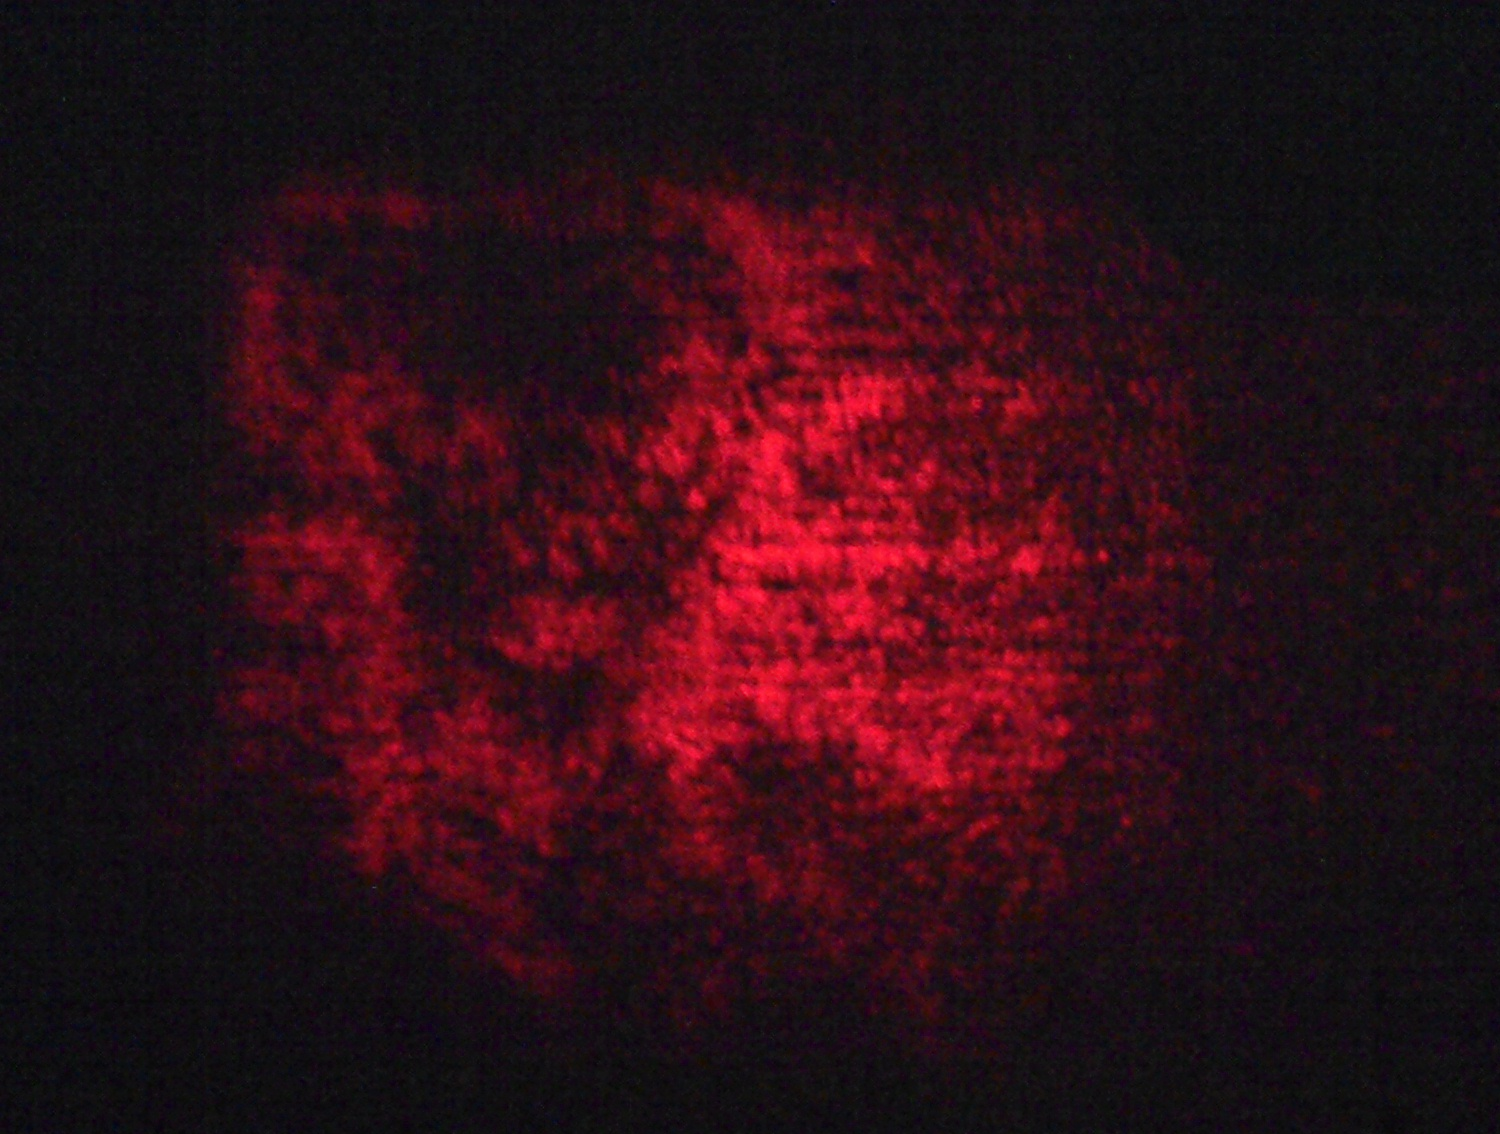
\includegraphics[width=\textwidth]{data/optics/06_Einstein_Dunkel_Bild}
		\caption{Dunkelfeld-Bild}				 \label{fig:Einstein_dunkel_B}
	\end{subfigure}
	\begin{subfigure}{0.49\textwidth}
		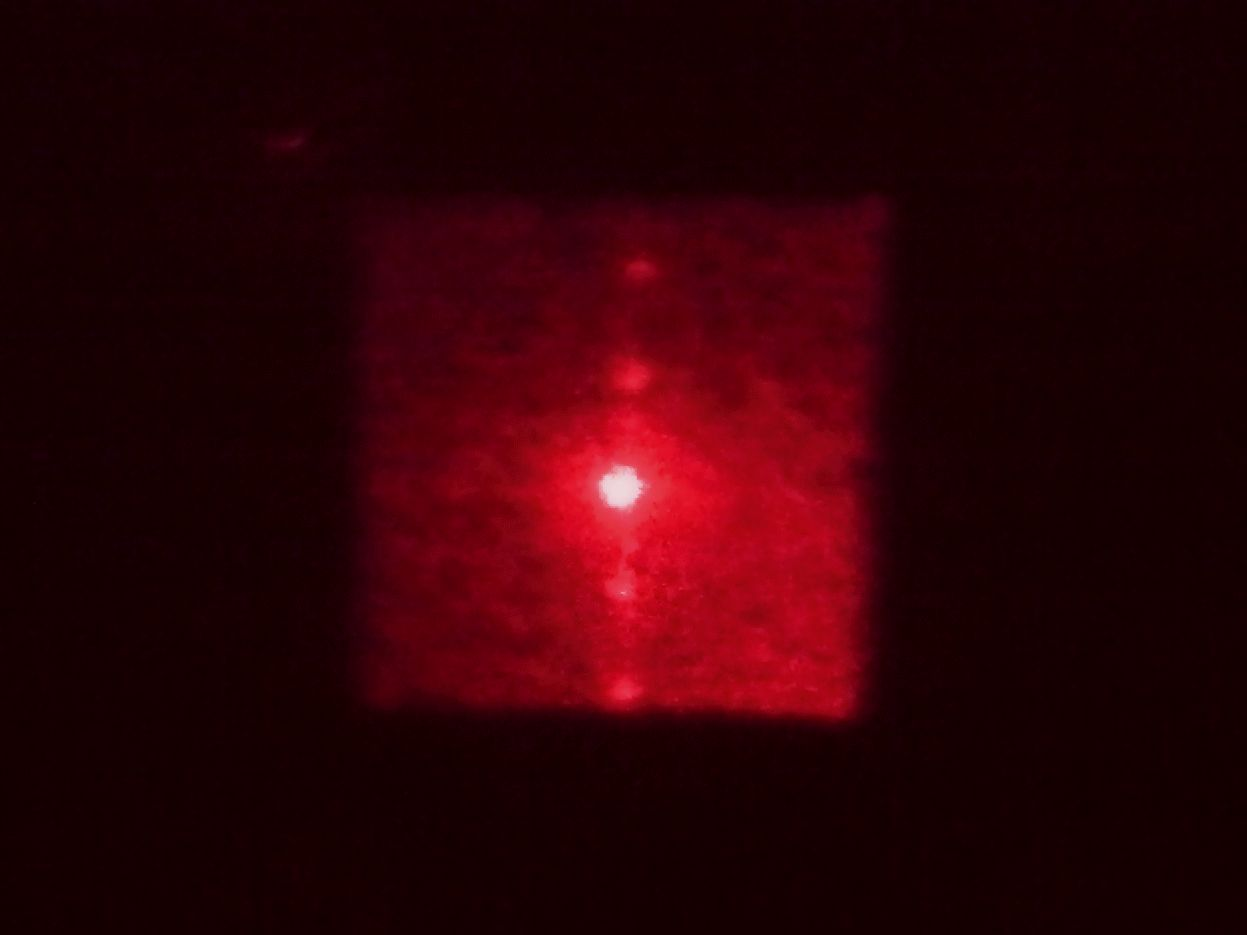
\includegraphics[width=\textwidth]{data/optics/06_Einstein_Dunkel_Beugung}
		\caption{Beugungsbild: Nebenmaximum}	 \label{fig:Einstein_dunkel_BG}
	\end{subfigure}
	\caption{Einstein-Portrait im Dunkelfeld}		\label{fig:Einstein_dunkel}
	\vspace{-5em}
\end{figure}




\newpage
\subsection{Transmissions-Elektronenmikroskop}
Das TEM ist analog zum Lichtmikroskop aufgebaut, wobei wir Elektronen anstelle von Photonen verwenden, da ihre De-Broglie-Wellenlänge
\begin{equation}
\lambda = \frac{h}{p} \stackrel{200\,\kilo\electronvolt}{=} 2,5\,\pico\metre
\end{equation}
ein deutlich höheres Auflösungsvermögen ermöglicht.

Der Versuchsaufbau ist in Abbildung \ref{fig:setup} dargestellt, die Linsen sind dabei als Magnetlinsen ausgeführt. Da letztere nur als Sammellinse (und nicht als Zerstreuungslinse) dienen können, sind die gewöhnlichen Korrekturen (z.B. Dubletts gegen chromatische Aberration) nicht anwendbar. Anstelle dessen wird das Energiespektrum der Elektronen eingeschränkt (Dispersion weniger relevant) und achsferne Strahlen durch zwei Multipole (Stigmatoren) korrigiert.


\begin{figure}[h]
	\centering
	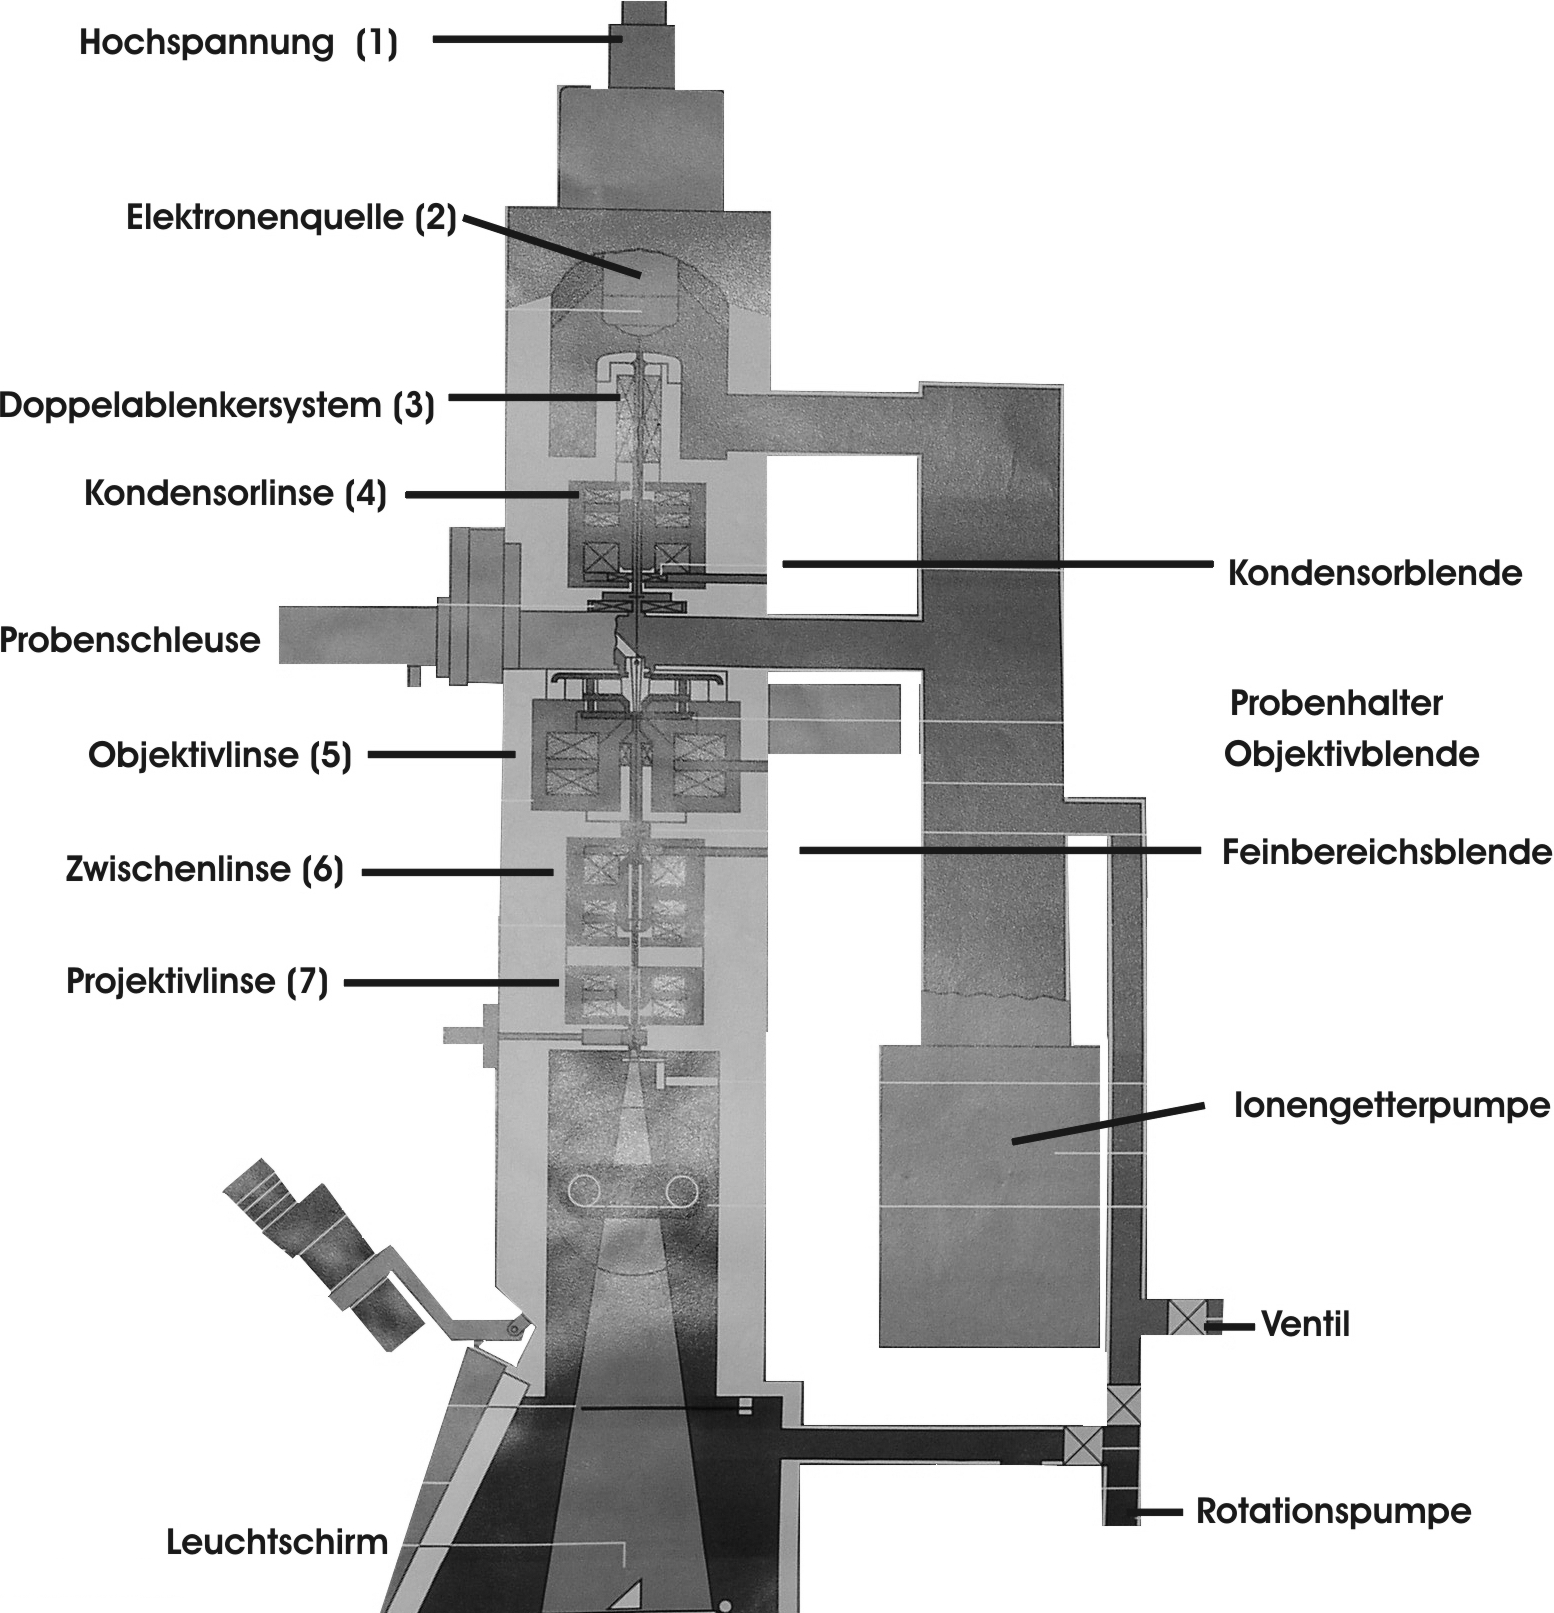
\includegraphics[width=0.75\textwidth]{Zeiss_TEM109.png}
	\caption{Querschnitt eines TEM (Zeiss TEM109) \cite{lit:tueb}}
	\label{fig:setup}
\end{figure}

\subsubsection{Unter-, Über-, Fokus}
Liegt die Probe exakt im Fokus der Objektivlinse, so wird sie ohne Interferenzeffekte abgebildet (Abb. \ref{fig:Fokus}). Eine Abweichung von dieser Einstellung wird  als Defokus bezeichnet und führt zu Fresnelsäumen im Bild: Bedingt durch Interferenz bilden sich an Kanten eine Streifenschar aus abwechselnd hellen und dunklen Bereichen.

Wird die Objektivlinse stärker angeregt, so verringert sich die Brennweite und das Objekt liegt unterhalb der Fokusebene. Diese Form der Defokussierung wird als Unterfokus bezeichnet und zeigt sich im Bild durch einen hellen ersten Saum am Rand der Probe  (Abb. \ref{fig:Unter}). Analog spricht man bei positivem Defokus von Überfokus und erkennt dies daran, dass der erste Fresnelsaum dunkel ist  (Abb. \ref{fig:Ueber}).
\begin{figure}[p]
	\vspace{-1.5em}
	\centering
	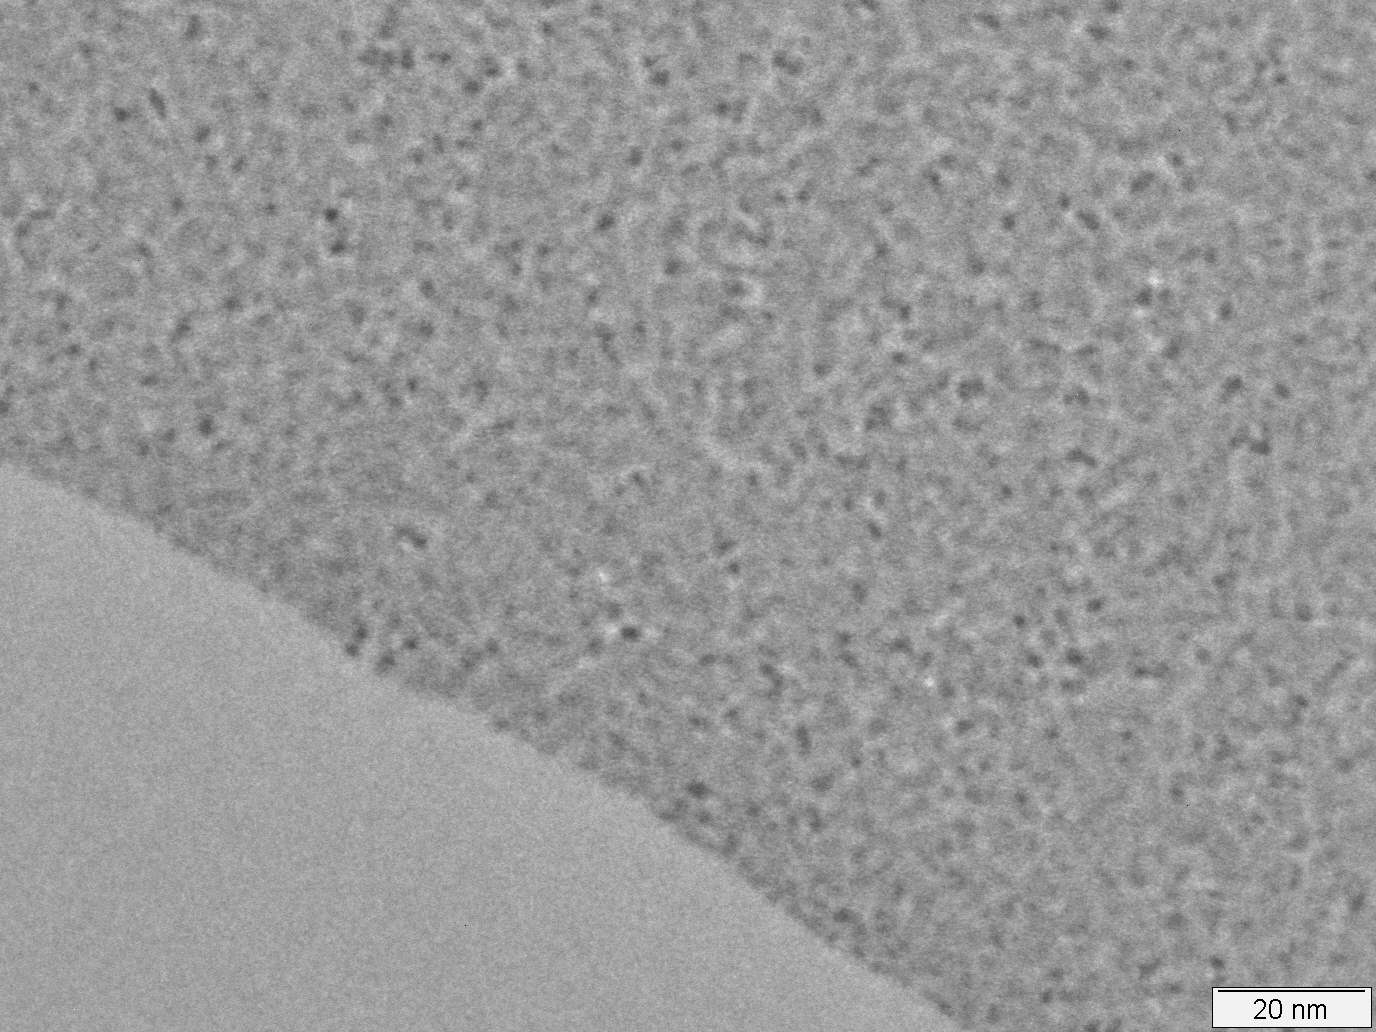
\includegraphics[width=0.68\textwidth]{data/Im_1.jpg}
	\vspace{-1.5ex}
	\caption{Rand einer Probe im Fokus, keine Fresnelstreifen}			\label{fig:Fokus}
	\vspace{-1em}
\end{figure}

\begin{figure}[p]
	\centering
	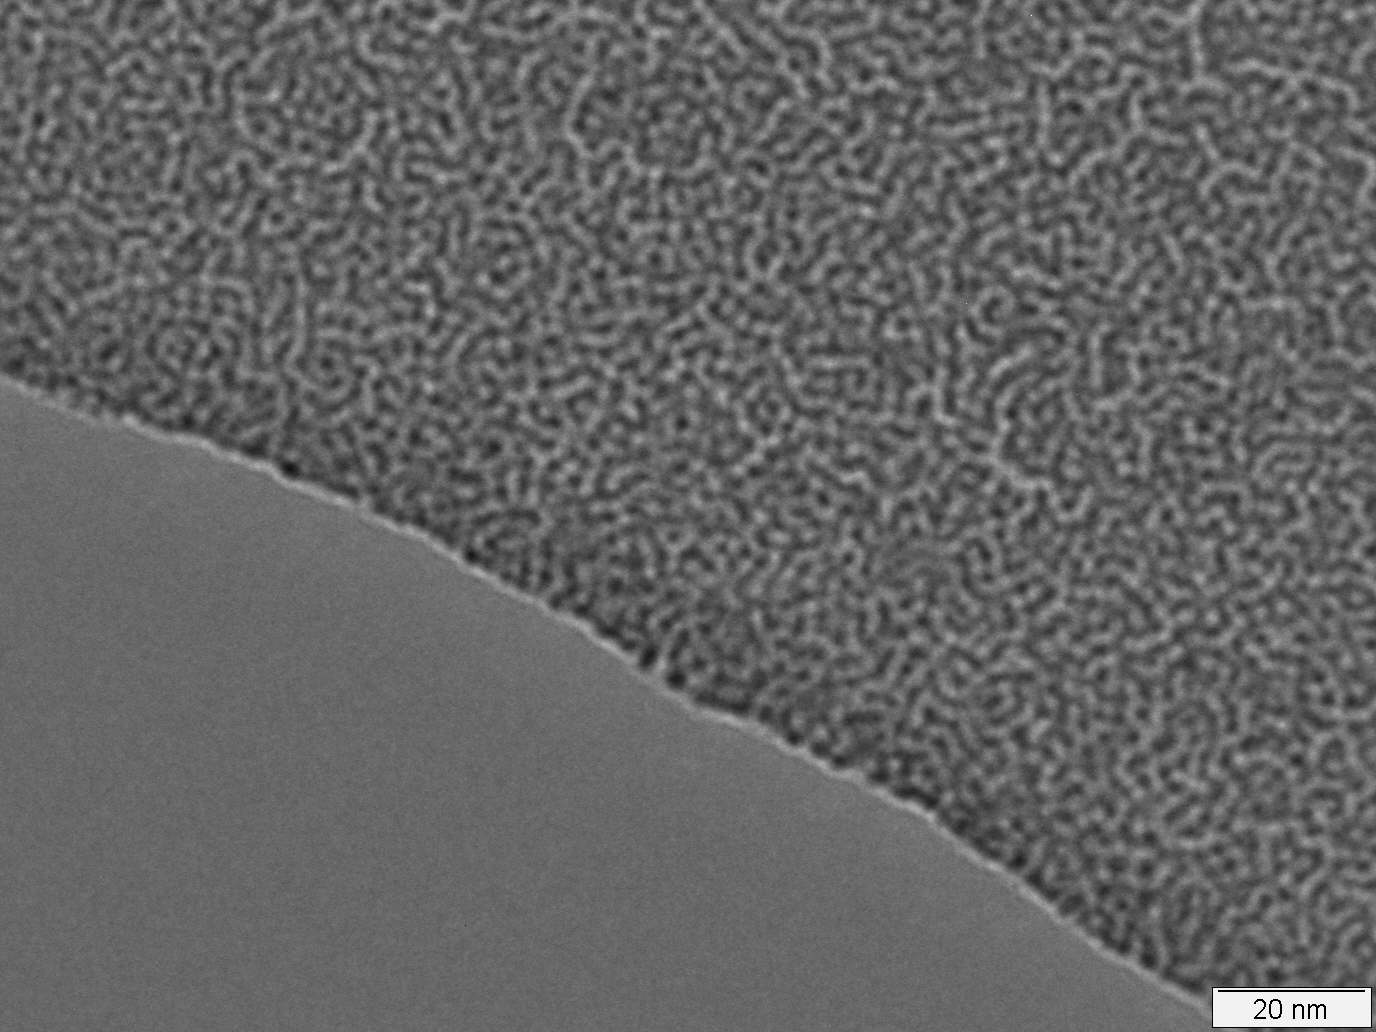
\includegraphics[width=0.68\textwidth]{data/Im_3.jpg}
	\vspace{-1.5ex}
	\caption{Rand einer Probe im Unterfokus, erster Fresnelsaum hell}		\label{fig:Unter}
	\vspace{-1em}
\end{figure}

\begin{figure}[p]
	\centering
	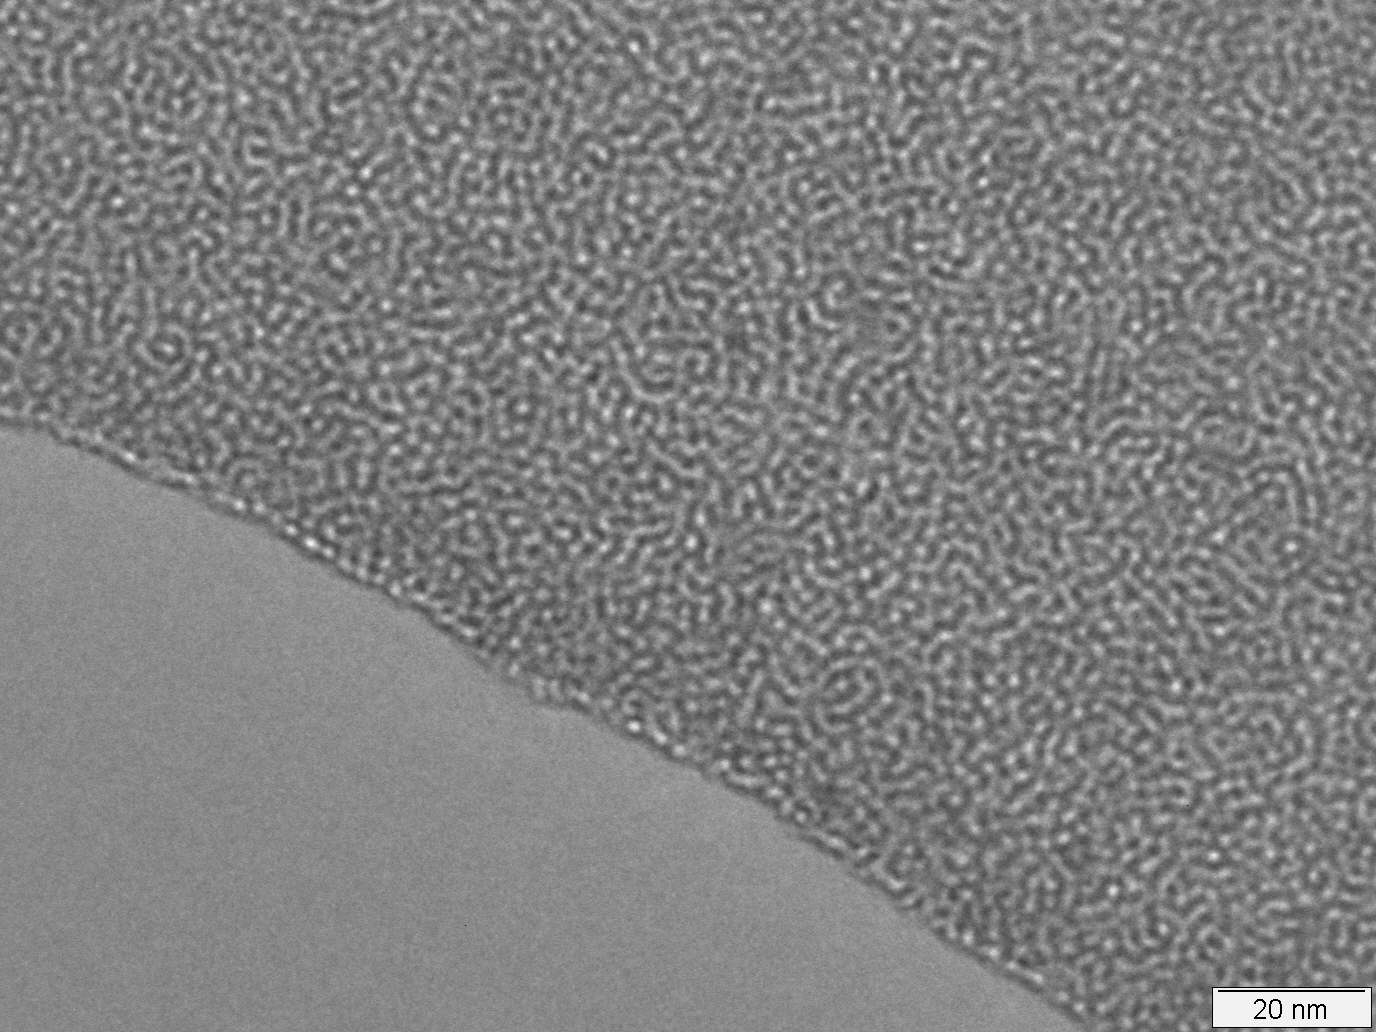
\includegraphics[width=0.68\textwidth]{data/Im_2.jpg}
	\vspace{-1.5ex}
	\caption{Rand einer Probe im Unterfokus, erster Fresnelsaum dunkel}	\label{fig:Ueber}
	\vspace{-9em}
\end{figure}

\subsubsection{Diffractogramm}
Das Diffractogramm ist die 2D-Fouriertransformation der Abbildung. Da die Qualität eines solchen errechneten Beugungsbildes geringer ist als eine Aufnahme im Beugungsmodus, wird in diesem Protokoll auf die Wiedergabe eines Diffractogramms verzichtet. Aus einer TEM-Aufnahme kann z.B. mit der Software ImageJ das Diffractogramm auch nachträglich berechnet werden.

% Diffractogramme nicht auf USB Stick dabei: freies Programm ImageJ, wahrscheinlich auch matlab (2D fft)

Normalerweise zeigt sich im Diffractogramm ein dunkler Ring, welcher zur Einstellung der Stigmatoren genutzt wird: Zweizähliger Astigmatismus führt zur Verzerrung dieses Rings zu einer Ellipse, bei korrekter Abstimmung der Spannungen an den Mutipolen erhält man wieder einen Kreis.

\subsubsection{}
High resolution (mehrere bilder mit Netz ebenen)
Im_5, Im_6
Meist nur eine Schar Netzebenen sichtbar (anstatt kariert) da die meisten Körner nicht in der fokusebene orientiert sind und somit nur eine Achse passt


Bright, Dark Field
Im_11 - Im_20
Brightfield: objektivblende lässt nur Hauptstrahl durch
Darkfield: ... nur Ausschnitt aus erstem beugungsRing durch
Zwei Bilder für unterschiedlichen Azimutwinkel --> unterschiedliche cluster leuchten auf (zwei verschiedene Orientierungen)



\subsubsection{}
Beugung (verdeckter Null Strahl zum Schutz der Kamera)

Beugung: gewisse ringe auf unterschiedlichen Bildern an besten sichtbar, überlagern (entweder nur Messwerte oder Bilder)
Bei 340mm Kamera abstand (30000x Vergrößerung)
300mm Schirm Abstand (26500x Vergrößerung)


2. Probe
- convergent beam (Kreise mit gebogenem Linien, geben Aufschluss über dicke der probe)
- Beugung, gleiche Einstellungen wie bei der ersten probe

110 Orientierung
1-1+-1, -11+-1, ..., 002, ..., 004 Reflexe zu sehen


Bei der ersten probe
Träger = Kupfernetz + Kohlenstoff-Folie
Probe = kristallines Pulver (durch verdunsten des lösungsmittels gleichmäßig verteilt)

Erste probe Edelmetall (zu bestimmen, vermutlich Gold), zweite probe Si Kristall


\begin{figure}[p]
	\centering
	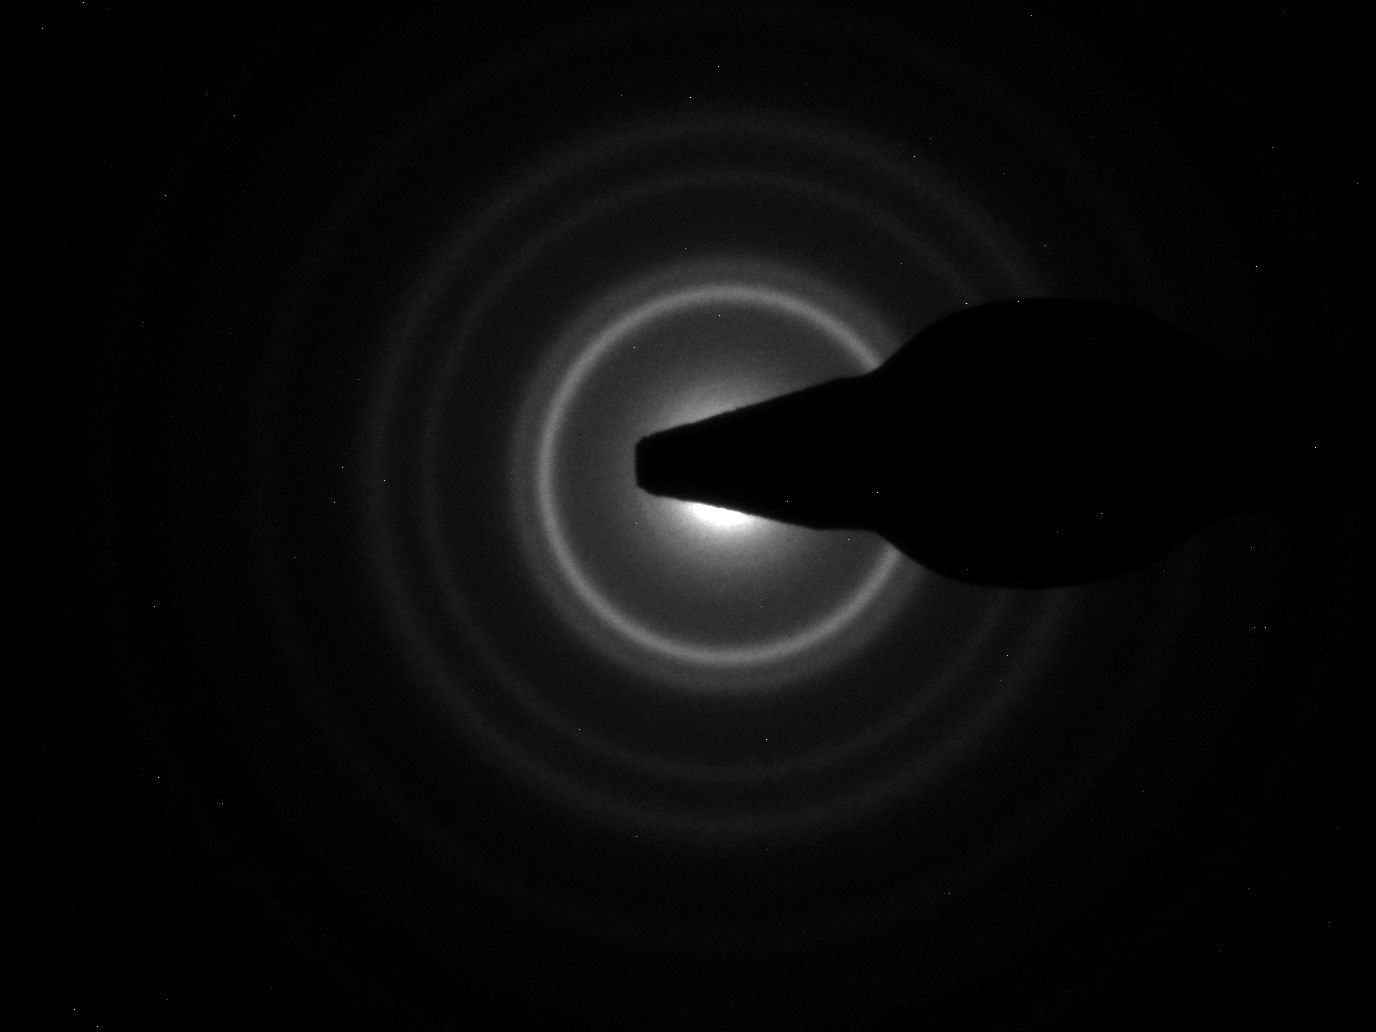
\includegraphics[width=0.9\textwidth]{data/Im_10.jpg}
	\caption{Beugungsbild des Edelmetall-Pulvers}		\label{fig:Edel}
\end{figure}

\begin{figure}[p]
	\centering
	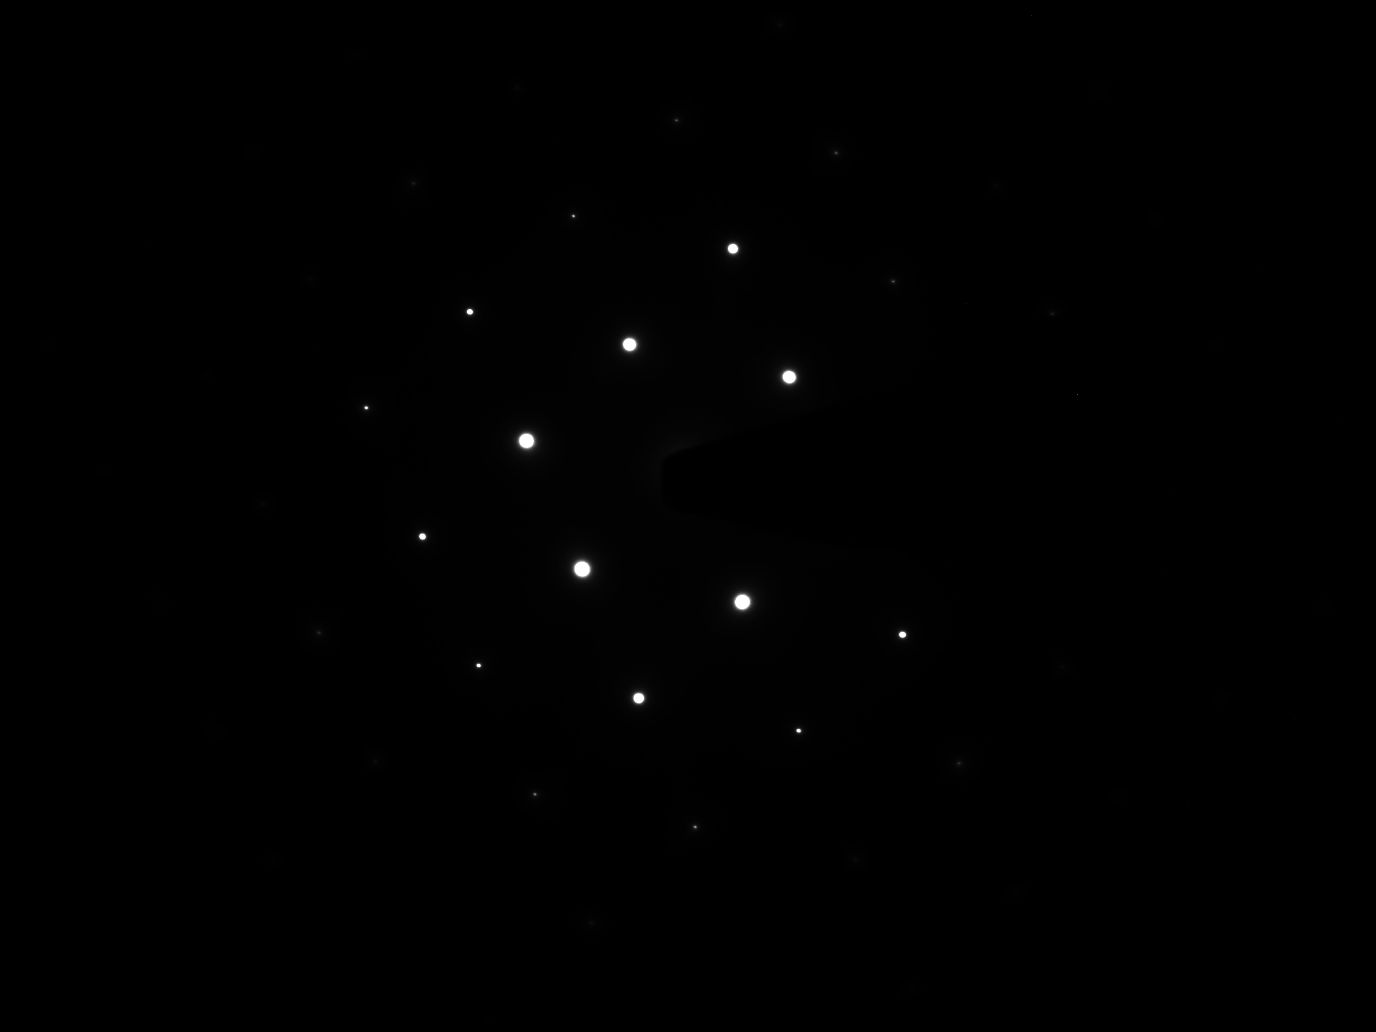
\includegraphics[width=0.9\textwidth]{data/Im_22.jpg}
	\caption{Beugungsbild des Silizium-Kristalls (110 Orientierung)}	\label{fig:Si}
	\vspace{-5em}
\end{figure}
